\documentclass[11pt]{article}
\usepackage[a4paper,margin=25mm]{geometry}
\usepackage{amsmath,amssymb,amsthm,mathtools}
\usepackage{booktabs,array,longtable}
\usepackage[dvipsnames]{xcolor}
\usepackage{hyperref,fancyhdr,graphicx}
\hypersetup{hypertexnames=false,colorlinks=true,linkcolor=MidnightBlue,urlcolor=MidnightBlue,citecolor=MidnightBlue,
pdftitle={Self-pinned distances through unforced scale selection}}
\setlength{\parindent}{0pt}\setlength{\parskip}{5pt}
\setlength{\emergencystretch}{2em}\setlength{\headheight}{14pt}
\pagestyle{fancy}\fancyhf{}\fancyhead[L]{\small Self-pinned distance sets}
\fancyhead[R]{\small Unforced scale selection}\fancyfoot[C]{\thepage}
\newtheorem{theorem}{Theorem}[section]
\newtheorem{proposition}[theorem]{Proposition}
\newtheorem{lemma}[theorem]{Lemma}
\theoremstyle{definition}\newtheorem{remark}[theorem]{Remark}
\newcommand{\R}{\mathbb R}\newcommand{\HH}{\dim_{\mathrm H}}\newcommand{\PP}{\dim_{\mathrm P}}
\newcommand{\supp}{\operatorname{supp}}\newcommand{\dist}{\operatorname{dist}}
\newcommand{\dd}{\,d}\newcommand{\norm}[1]{\left\|#1\right\|}\newcommand{\eps}{\varepsilon}

\begin{document}
\begin{titlepage}
\vspace*{18mm}
{\large\color{MidnightBlue} RESEARCH MANUSCRIPT}\par
\vspace{8mm}
{\Huge\bfseries Self-pinned distances}\par
\vspace{5mm}
{\LARGE through unforced scale selection}\par
\vspace{12mm}
30 September 2026
\vspace{12mm}

This manuscript refines the Hausdorff--packing sufficient condition by separating
standard spatial wave packets from the auxiliary angular partitions in the
Fourier estimate. The angular marks remain constant on each standard packet
label; only the spectral calculation is subdivided more finely. This removes
the prescribed midpoint from the scale-selection problem.

The latest refinement retains the location and height of a tail minimum,
and a second minimum on the preceding interval. Comparing several admissible
chains yields a further improvement for Hausdorff dimensions between
\(9/8\) and \(7/6\).

\textbf{Scope.} The manuscript gives the complete mathematical argument using
the explicitly cited established analytic inputs, including both analytic
branches and the Borel-set reduction. Internal checks are not external
refereeing or Lean kernel verification.

\textbf{Optimality.} The weakest possible condition on the two dimensions is
not established. An explicit profile proves sharpness of the upper-slope
unforced chain estimate in this method; it is not a planar distance-set
counterexample. No unrestricted improvement below the five-quarters threshold
is claimed.

\vfill
The existing Lean challenge and comparator are unchanged. This mathematical
manuscript does not complete the unconditional formalization.
\end{titlepage}
\tableofcontents
\clearpage
\section{Statement and scope}
For a Borel set \(E\subset\R^2\), write \(d=\HH E\), \(D=\PP E\), and
\(\Delta_y(E)=\{|x-y|:x\in E\}\). All distances are Euclidean and
\(|\cdot|\) denotes one-dimensional Lebesgue measure. The strongest sufficient
curve proved in this manuscript is
\begin{equation}\label{minimum:curve}
 B_{\rm M}(d)=\begin{cases}
 2d-1,&1<d\le\dfrac98,\\[7pt]
 1+b_*(d-1),&\dfrac98<d<\dfrac76,\\[7pt]
 \dfrac1{3-2d},&\dfrac76\le d\le\dfrac54.
 \end{cases}
\end{equation}
Here \(b_*(a)\) is the unique solution in \([2a,1/2]\) of
\(V(a,b)=a\), for the explicit rational minimum--maximum expression
\eqref{minimum:cost} below. The proof establishes uniqueness, continuity,
and the endpoint values \(b_*(1/8)=1/4\), \(b_*(1/6)=1/2\);
thus this definition requires no numerical or optimization hypothesis.

\begin{theorem}[Refined sufficient packing condition]\label{target:main}
Let \(E\subset\R^2\) be Borel. If \(1<d=\HH E\le5/4\) and
\(\PP E<B_{\rm M}(d)\), then \(|\Delta_y(E)|>0\) for some \(y\in E\).
\end{theorem}

The preceding, simpler sufficient curve remains useful for comparison:
\begin{equation}\label{uf:curve}
 B_{\rm U}(d)=\begin{cases}
 2d-1,&1<d\le\dfrac87,\\[7pt]
 \dfrac{2+2d-3d^2}{6-5d},&\dfrac87<d\le\dfrac76,\\[10pt]
 \dfrac1{3-2d},&\dfrac76<d\le\dfrac54.
 \end{cases}
\end{equation}
\begin{theorem}[Simpler sufficient packing condition]\label{target:unforced}
Let \(E\subset\R^2\) be Borel. If \(1<d=\HH E\le5/4\) and
$$
 \PP E<B_{\rm U}(d),
$$
then \(|\Delta_y(E)|>0\) for some \(y\in E\).
\end{theorem}
The proof constructs separated compact source and pin subsets of \(E\).
A source probability has absolutely continuous pinned distance measures for
almost every pin under the selected pin probability. Distance images of Borel
sets are analytic, hence Lebesgue measurable.

For example,
$$
 d=\frac{31}{25}=1.24\quad\Longrightarrow\quad
 D<\frac{25}{13}=1.923076923\ldots\ \text{ is sufficient}.
$$
At \(d=5/4\), the condition is \(D<2\); the equality case \(D=2\) is not
included. For \(d>5/4\), GIOW already gives the conclusion with no packing
restriction \cite{giow}. The endpoints of all branches in \eqref{uf:curve}
agree, and the packing inequality is strict throughout.

A new exact example is \(d=23/20=1.15\), \(D=27/20=1.35\).
The refined profile cost is \(187/1255\), giving the strict margin
\(1/1004\). The refined cutoff there is
\((37+\sqrt{13})/30=1.353518376\ldots\),
whereas \(B_{\rm U}(1.15)=1.33\) and the originally quoted cutoff was
\(1.30\). These decimal values illustrate the exact root definition;
they are not used in its proof.

\begin{figure}[ht]
\centering
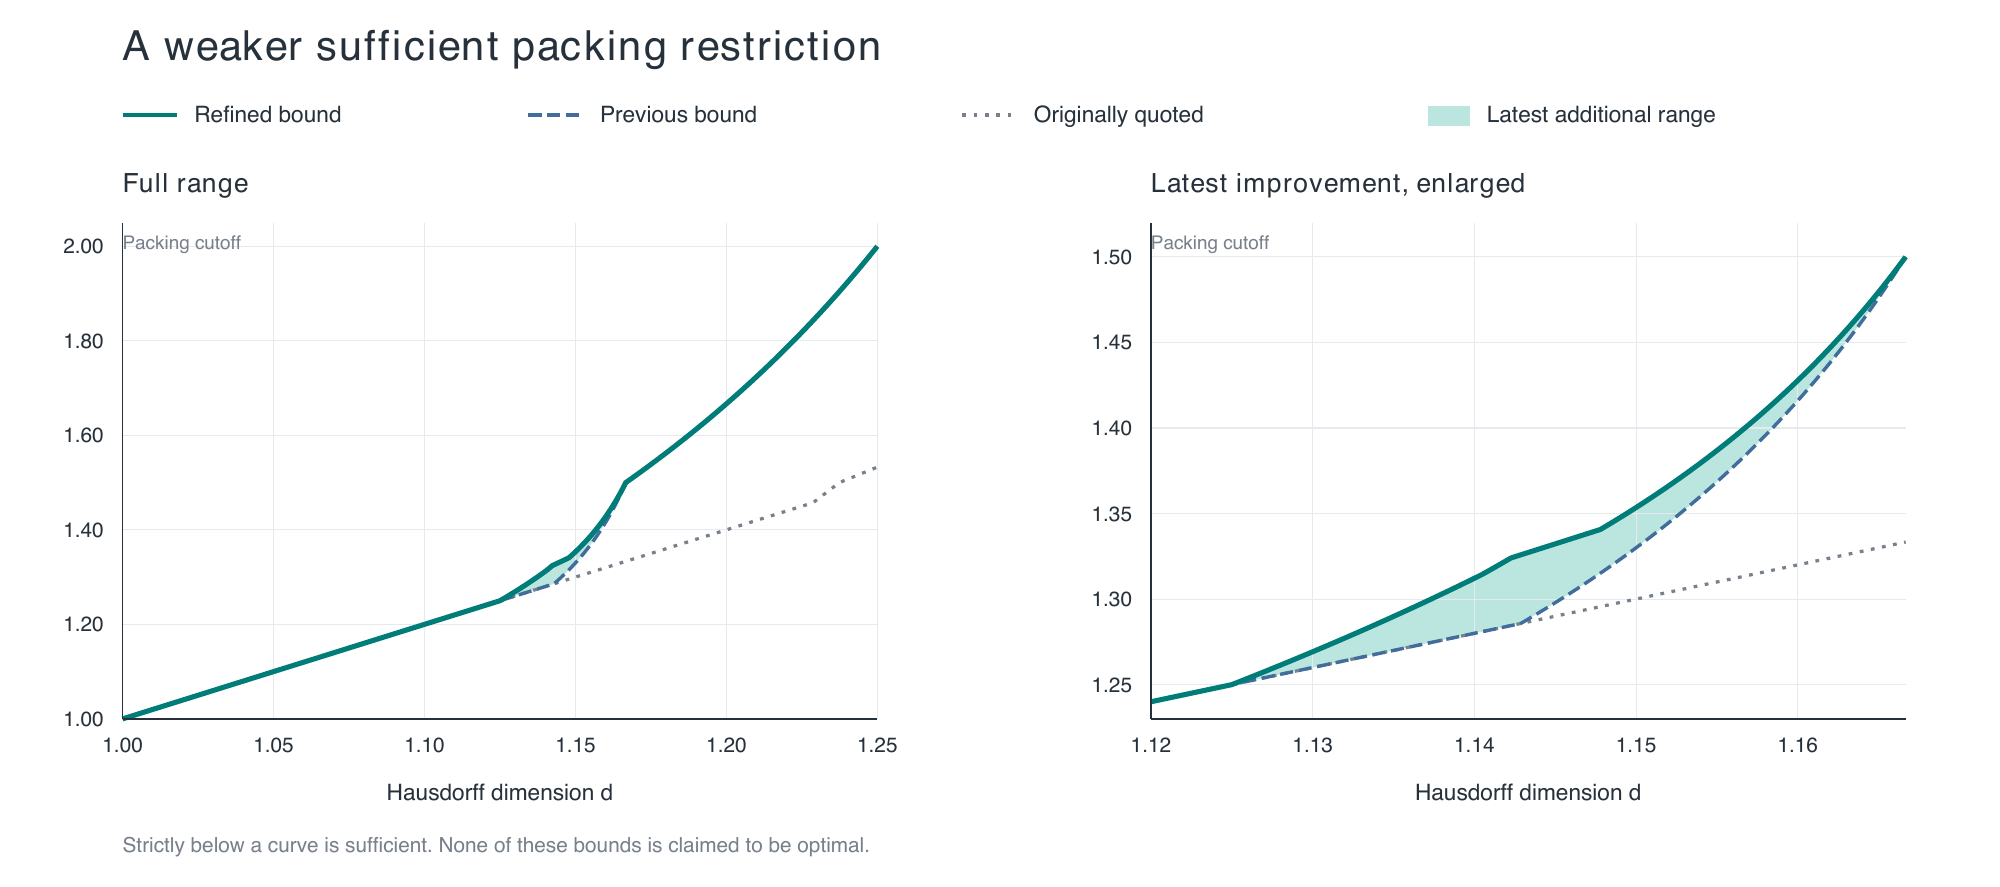
\includegraphics[width=\textwidth]{../figures/packing-unforced.png}
\caption{The refined sufficient curve, the preceding unforced curve, and the
originally quoted curve. The second panel isolates the latest improvement.
Values strictly below a curve are covered. No curve is asserted to be necessary.}
\end{figure}

\subsection{Definitions and established inputs}
A probability \(\mu\) is \(s\)-Frostman if
\(\mu(B(x,r))\le C r^s\) for \(0<r\le1\). Write
$$
 I_a(\mu)=\iint |x-x'|^{-a}\dd\mu(x)\dd\mu(x').
$$
An \(s\)-Frostman probability of bounded support has finite \(a\)-energy
whenever \(0<a<s\), by summing spatial annuli.
The external inputs are as follows.
\begin{enumerate}
\item Frostman's lemma for Borel subsets of Euclidean space, and the
countable bounded-cover characterization of packing dimension using upper box dimension.
Closures preserve bounded upper box dimension; positive-mass compact restrictions
are available by inner regularity.
\item Orponen's averaged radial-projection integrability \cite{orponen}, in the form
of GIOW Theorem 3.7 or Keleti--Shmerkin Theorem 3.11. For separated compact
Frostman probabilities of exponents greater than one, radial projections have
\(L^q\) densities for some \(q>1\), with integrable \(q\)-th powers of their norms.
\item Plancherel, the Riesz energy identity, polar coordinates and their projection
consequences, with Fourier normalization
\(\widehat f(\xi)=\int e^{-2\pi i x\cdot\xi}f(x)\,dx\).
\item Keleti--Shmerkin Lemma 3.4 and Corollary 3.5 \cite{ks}, used only for finite
terminal-cube restrictions, not to extract an infinite regular subset.
\item The elementary packet localization of GIOW Section 3 \cite{giow},
Liu's cap reconstruction (Lemma 4.2 of \cite{liu2026}), and the pinned quadratic
identity \cite{liuidentity}. The variable-chain inflation multiplier is derived below.
\end{enumerate}
All constants may depend on the fixed compact supports, positive source-pin
separation and chosen auxiliary parameters. They are uniform in frequency,
regularized component, cube and cap. The notation \(\operatorname{RapDec}(R)\)
means a quantity bounded by \(C_MR^{-M}\) for every fixed \(M>0\), uniformly
in those indices. Summing polynomially many such errors preserves this property.


\clearpage
\section{Coherent positive linearizations and a conditional convergence theorem}
\label{sec:coherenttree}

This section proves the original branch of the bound, rather than assuming Proposition E.6 from the longer report. It uses positive affine approximations to distance and a summable first-norm comparison.

\subsection{Angular regularity with a single exceptional set}

\begin{lemma}[Coupled-angle projection comparison]\label{lem:coherentangular}
Let \(0<\gamma<1/2\), and let \(\lambda\) be a probability supported in \(B(0,Cr)\), \(0<r\leq1\), with \(I_{1+2\gamma}(\lambda)<\infty\). For almost every \(\theta\in S^1\), let \(F(\theta)\in L^2(\R)\) be the density of \((\pi_\theta)_*\lambda\), where \(\pi_\theta(x)=x\cdot\theta\). There is a nonnegative function \(G\) with
$$
\|G\|_{L^2(S^1)}^2\leq C_\gamma r^{2\gamma}I_{1+2\gamma}(\lambda)
$$
such that, outside one angular null set, every pair satisfies
$$
\|F(\theta)-F(\phi)\|_{L^2(\R)}
\leq C_\gamma d(\theta,\phi)^\gamma\bigl(G(\theta)+G(\phi)\bigr),
$$
where \(d\) is circular arclength distance. In addition,
$$
\int_{S^1}\sup_{|v|\leq Cr^2}
\|F(\theta)(\cdot-v)-F(\theta)\|_2^2d\theta
\leq C_\gamma r^{4\gamma}I_{1+2\gamma}(\lambda).
$$
\end{lemma}
\begin{proof}
We first prove the Hilbert-valued angular Sobolev estimate
\begin{equation}\label{eq:coherentangularsobolev}
\|F\|_{H^\gamma(S^1;L^2(\R))}^2
\leq C_\gamma r^{2\gamma}I_{1+2\gamma}(\lambda).
\end{equation}
The projection-energy identity gives the projected densities and their joint second integrability, since finite \((1+2\gamma)\)-energy implies finite first energy on the bounded support. Fourier transform in the scalar projection variable. The transformed function is
$$
f_\tau(\theta)=\widehat\lambda(\tau\theta).
$$
Its angular derivative is a linear combination, with bounded angular coefficients, of \(\tau\widehat{x_k\lambda}(\tau\theta)\), \(k=1,2\). The Riesz energy identity for these signed measures gives
$$
\int_{\R^2}|\widehat{x_k\lambda}(\xi)|^2|\xi|^{2\gamma-1}d\xi
\leq C_\gamma r^2I_{1+2\gamma}(\lambda).
$$
Indeed the spatial double integral has the factor \(x_kx'_k\), whose absolute value is at most \(Cr^2\). Its absolute energy is finite, so approximation justifies the signed Fourier identity.

Angular Sobolev interpolation, or directly Holder on angular Fourier coefficients, gives
$$
\|f_\tau\|_{H^\gamma}^2
\leq\|f_\tau\|_2^{2(1-\gamma)}\|f_\tau\|_{H^1}^{2\gamma}.
$$
On \(|\tau|\geq1/r\), introduce the canceling weights
$$
A_\tau=|\tau|^{2\gamma}\|f_\tau\|_2^2,
\qquad
B_\tau=|\tau|^{-2(1-\gamma)}\|f_\tau\|_{H^1}^2.
$$
Polar coordinates and the preceding signed-energy estimate show
$$
\int_{|\tau|\geq1/r}A_\tau d\tau\leq C_\gamma I_{1+2\gamma}(\lambda),
\qquad
\int_{|\tau|\geq1/r}B_\tau d\tau\leq C_\gamma r^2I_{1+2\gamma}(\lambda).
$$
For the undifferentiated part of \(B_\tau\), use \(|\tau|^{-2}\leq r^2\); its derivative part has exactly the energy weight after the factor \(\tau^2\) is inserted. Holder in \(\tau\) now bounds the integral of \(\|f_\tau\|_{H^\gamma}^2\) by \(C_\gamma r^{2\gamma}I_{1+2\gamma}(\lambda)\) on this region. When \(|\tau|\leq1/r\), both \(f_\tau\) and its angular derivative are bounded uniformly, so the contribution is at most \(C/r\). This is absorbed because
$$
I_{1+2\gamma}(\lambda)\geq (Cr)^{-1-2\gamma}.
$$
Plancherel in the scalar variable proves \eqref{eq:coherentangularsobolev}.

Choose a measurable Hilbert-valued representative and define
$$
G(\theta)^2
=\int_{S^1}\frac{\|F(\theta)-F(z)\|_2^2}{d(\theta,z)^{1+2\gamma}}dz.
$$
The angular Slobodeckij identity gives \(\|G\|_2^2\leq C_\gamma\|F\|_{H^\gamma}^2\). For completeness, expand in angular Fourier coefficients: translation invariance makes each nonzero coefficient contribute its squared Hilbert norm times
$$
\int_{-\pi}^{\pi}\frac{|e^{ikh}-1|^2}{|h|^{1+2\gamma}}dh
\asymp_\gamma |k|^{2\gamma}.
$$
Tonelli and Parseval prove the assertion also for Hilbert-valued functions.

Remove the null set where \(G\) is infinite, where \(F\) is undefined, or where it does not represent the projected density. Given two remaining angles at distance \(\delta>0\), take an arc \(J\) of length comparable to \(\delta\) containing both, with every point of \(J\) within \(C\delta\) of each endpoint. Average the triangle inequality through \(z\in J\). Cauchy--Schwarz gives
$$
\begin{aligned}
\|F(\theta)-F(\phi)\|_2
&\leq |J|^{-1/2}
\left[\left(\int_J\|F(\theta)-F(z)\|_2^2dz\right)^{1/2}
+\left(\int_J\|F(\phi)-F(z)\|_2^2dz\right)^{1/2}\right]\\
&\leq C_\gamma\delta^\gamma\bigl(G(\theta)+G(\phi)\bigr).
\end{aligned}
$$
For large \(\delta\), the whole circle serves as \(J\); the diagonal case is immediate. This proves a single-null-set, all-pairs estimate, which can be evaluated on correlated angular laws.

Finally Plancherel bounds the translation expression, before angular integration, by
$$
Cr^{4\gamma}\int_\R |\tau|^{2\gamma}|\widehat\lambda(\tau\theta)|^2d\tau.
$$
Here the supremum over \(|v|\leq Cr^2\) was bounded inside the Fourier integral, using \(|e^{-2\pi i\tau v}-1|^2\leq C_\gamma|\tau v|^{2\gamma}\). Polar coordinates give the required translation bound.
\end{proof}

\subsection{Consecutive positive linearizations}

Let \(\mu,\nu\) be compact probabilities with positively separated supports, satisfying Frostman bounds with exponents \(s,t>1\). Choose
$$
0<\gamma<\min\left(\frac12,\frac{s-1}{2}\right).
$$
For a positive-mass dyadic source square \(Q\), write \(p_Q=\mu(Q)\), \(\mu_Q=p_Q^{-1}\mu|_Q\). Orponen's theorem, in the GIOW Theorem 3.7 form stated in the preliminaries \cite{orponen,giow}, supplies \(q>1\) and
$$
(\Theta_x)_*\nu=\rho_xd\sigma,\qquad
\Theta_x(y)=\frac{x-y}{|x-y|},\qquad
B=\int\|\rho_x\|_q^q d\mu(x)<\infty,
$$
where \(\sigma\) is normalized arclength. The hypotheses follow by choosing a common Frostman exponent between one and \(\min(s,t)\). In every node choose \(x_Q\in Q\cap\supp\mu\) at which the density exists and
$$
F_Q:=\|\rho_{x_Q}\|_q^q\leq\frac2{p_Q}\int_Q\|\rho_x\|_q^q d\mu(x).
$$
There are countably many nodes, and these choices give
$$
\sum_{Q\text{ at level }n}p_QF_Q\leq2B
\quad\text{at every level.}
$$
Define the affine approximation
$$
L_Q(x,y)=\Theta_{x_Q}(y)\cdot(x-y).
$$
At level \(n\), push the original positive pair probability by \((x,y)\mapsto(y,L_{Q_n(x)}(x,y))\). It has a nonnegative density \(f_n\) relative to \(\nu(dy)dt\). To see this, each \(\mu_Q\) has finite first energy and therefore second-integrable projected densities for almost every angle. Its chosen center's angular pin law is absolutely continuous, so the assertion holds for almost every pin, simultaneously at all countably many nodes. The conditional densities can be chosen jointly measurably. Each \(f_n\) has mass one, and Taylor's theorem gives
$$
|L_{Q_n(x)}(x,y)-|x-y||\leq C2^{-2n}
$$
uniformly, once the squares are smaller than the fixed separation.

\begin{proposition}[Coherent first-norm comparison]\label{prop:coherentcomparison}
For \(r=2^{-n}\) sufficiently small and every \(A\geq1\),
\begin{equation}\label{eq:coherentcomparison}
\|f_{n+1}-f_n\|_{L^1(\nu\times dt)}
\leq C\left[
A r^{1+4\gamma}\sum_{Q\text{ at level }n+1}p_QI_{1+2\gamma}(\mu_Q)
\right]^{1/2}+CB A^{1-q}.
\end{equation}
Constants depend on the fixed support geometry and separation, the exponents and Frostman bounds, but not on \(n,A\).
\end{proposition}
\begin{proof}
Let \(Q\) be a child of \(P\), and apply both affine maps to the same conditional source \(\mu_Q\). Set \(b=x_Q\), and recenter this source at \(b\). Put \(\theta=\Theta_{x_P}(y)\), \(\phi=\Theta_b(y)\). Their separation is \(O(r)\), and
$$
L_P(x,y)=\theta\cdot(x-b)+\theta\cdot(b-y),\qquad
L_Q(x,y)=\phi\cdot(x-b)+|b-y|.
$$
The constants differ quadratically:
$$
|\theta\cdot(b-y)-|b-y||
=|b-y|\,|\theta\cdot\phi-1|\leq Cr^2.
$$
Recentring is essential here; estimating the uncentered translations separately would lose a first-order term.

Keep those pins for which both angular densities at \(\theta\) and \(\phi\) are at most \(A\). The resulting joint angular law has both marginals bounded by \(A\sigma\), while its deleted pin mass is at most
$$
A^{1-q}(F_P+F_Q).
$$
No independence of the angles or of angular and radial pin coordinates is used. Apply Lemma \ref{lem:coherentangular} to the translated conditional source. Its pointwise all-pairs bound is valid on the coupled angles, since both marginals avoid the single exceptional null set. Integrating the square and using the marginal bounds gives \(CA r^{4\gamma}I_{1+2\gamma}(\mu_Q)\). The pin-dependent scalar translation has size at most \(Cr^2\); the lemma's translation estimate, with the relevant bounded angular marginal, gives the same bound. By the triangle inequality, the integrated squared second-norm difference of the two conditional affine densities is therefore at most
$$
CA r^{4\gamma}I_{1+2\gamma}(\mu_Q).
$$

For each pin both densities lie in a common interval of length \(Cr\). Cauchy--Schwarz converts their second norm to their first norm with factor \(Cr^{1/2}\). On deleted pins the first-norm difference of two probability densities is at most two. Decompose each parent conditional source into its children, sum with weights \(p_Q\), and use Cauchy--Schwarz over those weights and retained pins. The good terms give the square root in \eqref{eq:coherentcomparison}. The bad terms sum to at most \(CB A^{1-q}\), because
$$
\sum_Qp_QF_Q\leq2B,\qquad
\sum_{Q\text{ at level }n+1}p_QF_{\operatorname{parent}(Q)}
=\sum_{P\text{ at level }n}p_PF_P\leq2B.
$$
This proves the estimate.
\end{proof}

\subsection{The convergence criterion and its scope}

\begin{theorem}[Conditional-energy criterion]\label{thm:coherentcriterion}
Under the preceding assumptions, set
$$
Z_n=2^{-n(1+4\gamma)}
\sum_{Q\text{ at level }n+1}p_QI_{1+2\gamma}(\mu_Q),\qquad
\eta_q=\frac{q-1}{2q-1}.
$$
If \(\sum_n Z_n^{\eta_q}<\infty\), then \((d_y)_*\mu\) is absolutely continuous for \(\nu\)-almost every \(y\).
\end{theorem}
\begin{proof}
Enlarge \(B\) to at least one and omit finitely many scales so \(Z_n\leq1\). In Proposition \ref{prop:coherentcomparison} choose
$$
A_n=(B/\sqrt{Z_n})^{1/(q-1/2)}\geq1.
$$
Both terms are bounded by \(C B^{1/(2q-1)}Z_n^{\eta_q}\). Thus \(f_n\) is Cauchy in \(L^1(\nu\times dt)\). Its nonnegative limit has mass one. Uniform approximation of the affine maps to distance identifies its weak measure limit with the pushforward of \(\mu\times\nu\) by \((x,y)\mapsto(y,|x-y|)\). Uniqueness of disintegration then shows that, for almost every pin, the actual pinned law has the resulting density. In particular the conclusion is about the raw positive distance laws, not signed approximations.
\end{proof}

\subsection{The covering and Borel consequences}

\begin{proposition}[A covering-number sufficient condition]\label{prop:coherentcovering}
Suppose additionally that the number of occupied source squares of side \(r\) is at most \(Cr^{-u}\), uniformly for small dyadic \(r\). If \(u<2s-1\), then the preceding criterion holds for a suitable \(\gamma\). In particular an \(s\)-Ahlfors regular source, \(s>1\), satisfies this sufficient condition when the separated pin measure has a Frostman exponent greater than one.
\end{proposition}
\begin{proof}
For \(a<s\), integration of the source Frostman ball bound within a square of diameter \(O(r)\) gives, for each \(x\) in that square,
$$
\int_Q|x-x'|^{-a}d\mu(x')\leq C r^{s-a}.
$$
Integrate over \(x\in Q\) and normalize twice. This proves
$$
I_a(\mu_Q)\leq Cr^{s-a}/p_Q.
$$
Taking \(a=1+2\gamma<s\) and summing over occupied child squares yields
$$
\sum_Qp_QI_{1+2\gamma}(\mu_Q)\leq C r^{s-1-2\gamma-u},
\qquad Z_n\leq C r^{s-u+2\gamma}.
$$
The strict assumption \(u<2s-1\) permits a choice \(0<\gamma<\min(1/2,(s-1)/2)\) with \(s-u+2\gamma>0\). The series then converges geometrically. An \(s\)-Ahlfors regular support has covering number \(O(r^{-s})\), so one may take \(u=s\).
\end{proof}

For comparison, Keleti--Shmerkin \cite[Theorem 1.2]{ks} obtain full Hausdorff dimension of pinned distance sets when the source packing dimension is at most twice its Hausdorff dimension minus one. The absolute-continuity assertion below is derived from the preceding positive-density comparison; the cited dimension theorem is not an absolute-continuity input.

\begin{proposition}[Borel-set consequence]\label{prop:coherentborel}
Let \(E,F\subset\R^2\) be Borel sets such that
$$
\HH E>1,\qquad \PP E<2\HH E-1,\qquad \HH F>1.
$$
Then \(|\Delta_y(E)|>0\) for some \(y\in F\). More precisely, one can choose a compactly supported Frostman probability \(\mu\) on a compact subset of \(E\) so that, for any prescribed compactly supported \(t\)-Frostman pin probability \(\nu\) on \(F\), \(t>1\), the law \((d_y)_*\mu\) is absolutely continuous for \(\nu\)-almost every pin. The source measure here is a selected restriction, not an assertion about an arbitrary original measure on \(E\).
\end{proposition}
\begin{proof}
Choose \(1<s<\HH E\) and \(u>\PP E\) with \(u<2s-1\). Frostman's lemma gives an \(s\)-Frostman probability \(\mu_0\) compactly supported on \(E\). Choose \(u_0\) strictly between \(\PP E\) and \(u\). The countable-cover characterization of packing dimension gives a cover by bounded sets of upper box dimension at most \(u_0\). Replacing these sets by their closures preserves upper box dimension and makes them compact. At least one member has positive \(\mu_0\)-mass. By inner regularity, choose a compact subset \(K\) of its intersection with \(E\) having positive \(\mu_0\)-mass. Set \(\mu=\mu_0|_K/\mu_0(K)\). It is still \(s\)-Frostman, and its occupied-square count is \(O(r^{-u})\), since \(\overline{\dim}_{\rm B}K\leq u_0<u\).

It remains to remove the separation condition without changing this selected measure. Cover the complement of the diagonal in \(\R^2\times\R^2\) by countably many products of closed bounded rational balls \(U\times V\) with positive separation. The interiors of such products already cover the complement. On each positive-mass product, normalize the restrictions of \(\mu\) and the prescribed \(\nu\). These probabilities satisfy the Frostman and covering assumptions, have compact separated supports, and Proposition \ref{prop:coherentcovering} applies. Their joint pinned-distance pushforward is absolutely continuous with respect to \(\nu(dy)dt\).

The diagonal has \(\mu\times\nu\)-mass zero because \(\mu\) has no atoms. A set of zero \(\nu\times dt\)-measure therefore has zero preimage mass on every member of the countable cover and hence under the full pair probability. Its full joint distance law is absolutely continuous. Disintegration proves the claimed almost-everywhere pinned assertion. Since these laws have mass one and are supported on \(\Delta_y(K)\subset\Delta_y(E)\), their supports have positive length. Finally \(\HH F>1\) supplies a compactly supported pin Frostman probability with exponent greater than one.
\end{proof}

\clearpage
\section{The finite-profile branch}\label{fprof:section}

For \(1<s\le5/4\) and \(s\le u\le2\), define
\begin{equation}\label{fprof:A}
 C(s,u)=U(s-1,u-1),\qquad
 U(a,b)=\begin{cases}
 \dfrac{(b-a)(1-a)}{2(2b-a)},&a\le b\le1/2,\\[7pt]
 \dfrac{b-a}{1+2b},&1/2\le b\le1.
 \end{cases}
\end{equation}
The parameter \(a\) lies in \((0,1/4]\), so all denominators are positive.
The two expressions agree at \(b=1/2\).

\begin{theorem}[Finite-profile criterion]\label{fprof:main}
Let \(E\subset\R^2\) be Borel, and write \(d=\HH E\), \(D=\PP E\). If
\begin{equation}\label{fprof:condition}
 1<d\le5/4,\qquad C(d,D)<d-1,
\end{equation}
then \(|\Delta_y(E)|>0\) for some \(y\in E\).
\end{theorem}

\subsection{The profile optimization}

If \(g\) is a continuous function on \([0,N]\), put
$$
 c_g(m,n)=g(m)-\min_{m\leq x\leq n}g(x),\qquad 0\leq m<n\leq N.
$$
The direction of this difference matters: the left endpoint is the larger physical cell. Call an edge \([m,n]\) admissible if \(2n-m\leq N\).

\begin{lemma}[A bounded-length chain]\label{fprof:chain}
Let \(N\) be a positive integer. Suppose \(g(0)=0\), \(g\) is 1-Lipschitz and piecewise linear on the integer grid, and
$$
 ax\leq g(x)\leq bx,\qquad
 0<a\leq b\leq1,\quad b\geq\tfrac12.
$$
Given an integer \(0\leq n_0<N\), there is an admissible decreasing chain from \(n_0\) to zero, of at most
$$
 3\left\lceil\log_2\frac{N}{N-n_0}\right\rceil+5
$$
edges, with total cost at most \((bN-g(N))/(1+2b)+3\).
On a grid of mesh \(T\), replace the additive constant by \(3T\).
\end{lemma}
\begin{proof}
Define
$$
 L(x)=2bx-bN-g(x),\qquad V(x)=\frac{\max\{L(x),0\}}{1+2b}.
$$
The function \(L\) is nondecreasing. On \(\{L\geq0\}\), almost everywhere,
$$
 (-g')_+\leq\frac{2b-g'}{1+2b}.
$$
For \(g'\geq0\) this follows from \(2b\geq1\); for \(g'<0\) it is equivalent to \(g'\geq-1\). Also
$$
 c_g(m,n)\leq\int_m^n(-g')_+\,dx.
$$
Let \(q\) be the largest integer with \(L(q)\leq0\). From \(n_0>q+1\), repeatedly replace \(n\) by \(\max\{q+1,2n-N\}\). These admissible edges double \(N-n\), except possibly the last. Their total cost is at most \(V(n_0)-V(q+1)\). If required, the edge from \(q+1\) to \(q\) costs at most one. If \(n_0\leq q\), omit this part.

In the region \(L\leq0\), for \(n>N/2\) set \(m_0=2n-N\). Then
$$
 g(m_0)\leq bm_0\leq g(n).
$$
Choose the leftmost grid minimum on \([m_0,n]\). It occurs before \(n\), gives a zero-cost admissible edge, and remains in \(L\leq0\). If \(n\leq N/2\), the edge to zero has zero cost since \(g\geq0\). Thus a finite zero-cost continuation exists. Merge consecutive edges greedily whenever their union is admissible. Their union still has zero cost. Maximality implies that every two merged edges more than double \(N-n\), except at the end. This gives the stated edge count. Finally \(V(n_0)\leq V(N)=(bN-g(N))/(1+2b)\). Rescaling proves the mesh version.
\end{proof}

\subsection{The unforced scale-profile estimate}
\label{unforced:profile-section}

An edge from \(n\) to \(m<n\) in \([0,N]\) is admissible when
\(2n-m\le N\), and its cost is
$$
 c_g(m,n)=g(m)-\min_{[m,n]}g.
$$
No intermediate endpoint is prescribed in this section. This distinction is
essential: the following estimate can be used in a distance argument only after
the analytic transfer has been justified for such unforced chains.

\begin{lemma}[Unforced profile bound]\label{unforced:profile}
Let \(0<a\le b\le1\), and let \(g:[0,N]\to\mathbb R\) be 1-Lipschitz
with \(ax\le g(x)\le bx\). For every \(0\le n_0<N\), an admissible
decreasing chain from \(n_0\) to zero exists with at most
$$
 K\le C\left(1+\log\frac{N}{N-n_0}\right)
$$
edges and total cost at most \(NU(a,b)\), where
\begin{equation}\label{unforced:cost}
 U(a,b)=\begin{cases}
 \dfrac{(b-a)(1-a)}{2(2b-a)},&b\le1/2,\\[7pt]
 \dfrac{b-a}{1+2b},&b\ge1/2.
 \end{cases}
\end{equation}
The formulas agree at \(b=1/2\). On a grid of mesh \(T\) containing
\(0,n_0,N\), the endpoints can be chosen on the grid with additional
\(O(KT)\) cost. If the barriers hold with uniform additive error
\(\epsilon N\), the additional cost is \(O(K\epsilon N+KT)\).
\end{lemma}

\begin{proof}
The case \(b\ge1/2\) is the bounded-length unforced chain estimate of
Lemma~\ref{fprof:chain}, followed by the grid limit described below. We prove the additional case \(b\le1/2\),
normalizing \(N=1\). Set
$$
 q=\frac{b}{2b-a},\qquad r=2q-1=\frac{a}{2b-a}.
$$
Then \(1/2<q\le1\) and \(0<r\le1\).

First observe that every endpoint \(n\le q\) admits free continuation
to zero. For \(1/2<n\le q\),
\begin{equation}\label{unforced:zero-zone}
 g(2n-1)\le b(2n-1)\le an\le g(n),
\end{equation}
because \((2b-a)n\le b\). Choosing the leftmost minimum of \(g\)
on \([2n-1,n]\) gives an admissible zero-cost edge with endpoint less
than \(n\). When \(n\le1/2\), the edge directly to zero is admissible
and costs zero since \(g(0)=0\) and \(g\ge0\). On a finite grid the
procedure terminates. Consecutive zero-cost intervals can be merged whenever
their union is admissible, and their union remains zero-cost. Every two
consecutive unmergeable intervals more than double the complementary depth,
so the retained zero-cost chain has the required logarithmic length.
If \(a=b\), then \(q=1\), and this argument already proves the result
with zero cost. It also handles any starting point \(n_0\le q\).

For the remaining initial portion, define on \([r,1]\)
$$
 H(z)=\frac z2+\left(b-\frac12\right)r.
$$
This majorizes \(bz\), since
$$
 H(z)-bz=\left(\frac12-b\right)(z-r)\ge0.
$$
For \(x\ge q\), put
$$
 \Lambda(x)=H(2x-1)-g(x)
 =x-\frac12+\left(b-\frac12\right)r-g(x).
$$
The function \(\Lambda\) is nondecreasing, and
$$
 \Lambda(q)=H(r)-g(q)=br-g(q)=aq-g(q)\le0.
$$
Almost everywhere,
$$
 (-g')_+\le\frac{1-g'}2=\frac{\Lambda'}2.
$$
Use maximal admissible downward jumps through \(\{\Lambda>0\}\),
shortening the last jump if necessary to reach its lower boundary. Their
costs sum to at most \(\Lambda(n_0)_+/2\), because each edge cost is
bounded by the negative variation of \(g\) over its interval. This is at
most \(\Lambda(1)/2\).

For a subsequent endpoint \(n\ge q\) with \(\Lambda(n)\le0\), the
majorant is valid at \(2n-1\ge r\), and gives
$$
 g(2n-1)\le H(2n-1)\le g(n).
$$
Choose a leftmost minimum on \([2n-1,n]\) to take a zero-cost edge.
Continue until the endpoint becomes at most \(q\); it need not equal
\(q\). Below \(q\), use \eqref{unforced:zero-zone} to continue for free.
The maximal jumps in the positive region double complementary depth except
at the last jump. Compressing the zero-cost intervals as above gives the
claimed bound on the total number of edges.

Finally, \(H(1)\ge g(1)\ge a\), and therefore
$$
 \frac{\Lambda(1)}2
 \le\frac{1/2+(b-1/2)r-a}{2}
 =\frac{(b-a)(1-a)}{2(2b-a)}.
$$
This proves the cost bound.

For precision about arbitrary continuous profiles, first run the construction
on piecewise affine interpolants on grids with mesh tending to zero.
The interpolants retain both barriers and the Lipschitz constant. If
\(n_0\) is not a grid point, first jump to the nearest grid point below
it; for sufficiently small mesh this is admissible and costs at most the
mesh. Rounding
the potential sign change and the threshold \(q\) requires at most a
bounded number of grid crossings, each costing \(O(T)\). For example,
one stops the positive-potential construction at the first grid point above
its lower boundary, then takes the adjacent grid edge across that boundary.
Below \(q\), the barrier argument applies directly. The edge-count bound
is independent of the mesh. Pad endpoint lists by repeated endpoints and
extract a convergent subsequence. Interval minima vary continuously with
the profile and endpoints, and admissibility is closed. Removing repeated
endpoints gives the exact continuous statement. This also proves the
asserted fixed-mesh error bound.

For approximate barriers, clamp the profile between \(ax\) and \(bx\)
and interpolate its grid values. This preserves the 1-Lipschitz property
and changes the profile uniformly by \(O(\epsilon N+T)\). Every edge
cost changes by at most twice this amount. The resulting total error is
\(O(K\epsilon N+KT)\), as claimed.
\end{proof}

The improvement over the global slope-\(1/2\) majorant is quantified by
$$
 \frac{1/2-a}{2}-U(a,b)
 =\frac{a(1/2-b)}{2(2b-a)}\ge0\qquad(b\le1/2).
$$
The gain is strict below \(b=1/2\). This estimate is not asserted to be
optimal in the small-slope range.


\subsection{Finite regularization of the original pin measure}

The constants in losses \(R^{C_Kh}\) below are independent of the
regularization block size \(T\); fixed annular ratios depending on
\(T\) change only multiplicative constants.

We prove a measure version of Theorem~\ref{fprof:main}. Let \(\mu,\nu\) be probabilities on separated compact sets, normalized by a common translation and dilation into the interior of one unit
dyadic cube. This preserves positive source-pin separation and both dimension
exponents. Suppose both are \(t\)-Frostman for some \(t>s>1\), and
\begin{equation}\label{fprof:cover}
 N(\supp\nu,r)\leq C r^{-u},\qquad 0<r\leq1.
\end{equation}
We will prove
\begin{equation}\label{fprof:ac}
 C(s,u)<s-1\quad\Longrightarrow\quad
 (d_y)_*\mu\ll\mathcal L^1\quad\text{for \(\nu\)-almost every \(y\)}.
\end{equation}
Constants can depend on these fixed measures and their separation. The radial-projection theorem of Orponen, in the form of GIOW Theorem 3.7 or Keleti--Shmerkin Theorem 3.11, supplies \(q>1\) such that
\begin{equation}\label{fprof:radial}
 B=\int\|\pi^y_*\mu\|_{L^q(S^1)}^q\dd\nu(y)<\infty.
\end{equation}
Here \(\pi^y(x)=(x-y)/|x-y|\). We also have \(I_s(\mu)<\infty\).

Fix a large integer \(T\). Use a smooth partition of frequency space into a low-frequency ball and annuli indexed by \(R=2^N\), \(N=4T\ell\). The annular ratios depend only on \(T\); all localization constants below may do so as well. Write \(P_R\) for the annular multiplier, including a fixed smooth spatial cutoff equal to one near \(\supp\mu\) and supported a positive distance from \(\supp\nu\). These multipliers have uniformly bounded convolution-kernel first norms, with constants depending on \(T\).

Apply Keleti--Shmerkin's finite regularization, Lemma 3.4 and Corollary 3.5, at depth \(N\). More precisely, first distribute each depth-\(N\) cube mass uniformly within that cube. The lemma partitions all but mass \(2^{-\epsilon N}\) into disjoint unions \(X_i\) of terminal cubes. Retain the \emph{original} restrictions
$$
 w_i=\nu(X_i),\qquad \sigma_i=w_i^{-1}\nu|_{X_i}.
$$
They have the same coarser cube masses as the regularized measures. With
$$
 \Gamma=\epsilon+\frac{\log_2(4T+2)+2}{T},
$$
we have \(w_i\geq R^{-\Gamma}\). For each \(i\), a function \(f_i\), linear on the \(T\)-grid with slopes in \([0,2]\), satisfies \(f_i(0)=0\) and, for every occupied cube of block depth \(k\),
\begin{equation}\label{fprof:masses}
 2^{-f_i(k)-N/T}\leq\sigma_i(Q)\leq2^{-f_i(k)}.
\end{equation}
This follows directly by multiplying the one-step mass ratios in the definition of a regular measure. Also
\begin{equation}\label{fprof:barriers}
 sk-C\Gamma N-C_T\leq f_i(k)\leq uk+C_T.
\end{equation}
For the first inequality use \(\sigma_i\leq R^\Gamma\nu\), the Frostman bound, and the lower estimate in \eqref{fprof:masses}. For the second, the upper estimate in \eqref{fprof:masses} forces at least \(2^{f_i(k)}\) occupied cubes, whereas \eqref{fprof:cover} bounds their number by \(C2^{uk}\). Interpolation extends the barriers with \(O(T)\) error. Finally,
\begin{equation}\label{fprof:radialcomponent}
 \int\|\pi^y_*\mu\|_q^q\dd\sigma_i(y)\leq B R^\Gamma.
\end{equation}

Put \(g_i=f_i-\mathrm{id}\). Apply Lemma~\ref{unforced:profile} with
\(a=s-1\), \(b=u-1\). Start at the \(T\)-grid point immediately
below \((1-\zeta)N\), where \(0<\zeta<1/8\) is fixed.
We obtain a chain, common to the entire component,
\begin{gather}\label{fprof:levels}
 n_0>n_1>\cdots>n_K=0,\qquad 2n_j-n_{j+1}\le N,\\
 K\le C\log(1/\zeta)+C,\qquad
 \sum_{j<K}c_{i,j}\le C(s,u)N+C K\Gamma N+C_{T,K},\label{fprof:sumcost}\\
 c_{i,j}=g_i(n_{j+1})-\min_{[n_{j+1},n_j]}g_i.\nonumber
\end{gather}
No intermediate endpoint is prescribed. Admissibility of the final edge implies
\(n_{K-1}\le N/2\), which is all that the final Fourier estimate will need.
Grid interpolation in the clamping step only changes the last constant. The source \(\mu\) is never restricted or regularized in this process.

\subsection{Truncated conditional energies and deletion}

For one edge write \(m=n_{j+1}\), \(n=n_j\), \(b=2^{-m}\), \(a=2^{-n}\), and \(\rho=a/b\). A cube is called active when its \(\sigma_i\)-mass is positive. Only active cubes and their ancestors occur below.

Let \(Q\) be an active depth-\(m\) cube. For any concentric enlargement \(Q^+\) by a factor between one and \(R^{C_Kh}\), set \(\lambda=(\sigma_i)_{Q^+}\). For \(m\leq k\leq n\), covering a ball by boundedly many dyadic cubes and using \eqref{fprof:masses} gives
$$
 \lambda(B(z,2^{-k}))\leq C R^{C\Gamma}2^{f_i(m)-f_i(k)}.
$$
Indeed, the denominator is at least the mass of the original active cube \(Q\); this avoids any boundary-sliver assumption about \(Q^+\). For intermediate radii between consecutive block-grid points, use the mass
bound at the coarser grid point. The ratio between adjacent radii is at most
\(2^T\), so this changes the estimate by a multiplicative constant depending
only on \(T\) (one may take \(O(2^{2T})\)). It introduces no additional power
of \(R\). Summing dyadic annuli yields
\begin{equation}\label{fprof:energy}
 J_\lambda(\rho):=\iint\min\{\rho^{-1},b/|y-z|\}\dd\lambda(y)\dd\lambda(z)
 \leq C(N+1)R^{C\Gamma}2^{c_{i,j}}.
\end{equation}
For separations larger than \(b\), use the bound one. For the other annuli the summand is at most
$$
 C R^{C\Gamma}2^{k-m+f_i(m)-f_i(k)}
 =C R^{C\Gamma}2^{g_i(m)-g_i(k)}.
$$
The innermost ball satisfies the same estimate. Replacing \(b\), the tube width, or the truncation parameter by factors at most \(R^{C_Kh}\) changes \eqref{fprof:energy} by at most another factor \(R^{C_Kh}\). This follows directly from the minimum kernel; no infinite conditional energy is used.

Here is the deletion argument with its multiplier exposed. If a probability \(\lambda\) is in a ball of radius \(b\), take a \(\rho\)-net of unoriented directions and, in each direction, a bounded-overlap cover by \(\rho b\)-wide tubes. Pair counting gives
\begin{equation}\label{fprof:pairs}
 \sum_T\lambda(T)^2\leq C J_\lambda(\rho).
\end{equation}
For fixed \(y,z\), at most
\(C\min\{\rho^{-1},b/|y-z|\}\) directions can place both points in such a tube; the spatial tube multiplicity in one direction is bounded. Integrating this statement proves \eqref{fprof:pairs}. Enlarged supports and tubes introduce only powers of the enlargement factor.

For each pin, delete source directions whose angular maximal density exceeds a threshold \(L\). The maximal inequality on the circle and Holder's inequality imply
\begin{equation}\label{fprof:sourcebad}
 (\mu\times\sigma_i)(\text{source-heavy pairs})
 \leq C_q L^{1-q} B R^\Gamma.
\end{equation}
For completeness, if \(v_y\) is the angular density, then
\(\int_{\{Mv_y>L\}}v_y\leq C_qL^{1-q}\|v_y\|_q^q\): bound the length of that set by \(C_qL^{-q}\|v_y\|_q^q\), then use Holder. Intervals centered at a retained direction therefore have mass at most a constant times their length times \(L\).

Now declare a pin tube heavy when \(\lambda(T)>H\rho\). Associate to it the unit-length source tube in the same direction, widened to angular width \(C\rho\). If this tube contains any pair not source-heavy, its source mass is at most \(CL\rho\). The fixed source-pin separation justifies this correspondence. Consequently the retained mass of pairs using heavy pin tubes is at most
\begin{equation}\label{fprof:pinbad}
 CL\rho\sum_{\lambda(T)>H\rho}\lambda(T)
 \leq \frac{CL}{H}\sum_T\lambda(T)^2
 \leq \frac{CL}{H}J_\lambda(\rho).
\end{equation}
One can discretize all tube centers and directions here: replacing a tube by a containing member of a grid changes widths by fixed factors. Directions within \(O(\rho)\) have the same containing tube after this enlargement. Thus the estimate also bounds the union over the finer angular caps used below, without paying their number.

Sum \eqref{fprof:pinbad} over active parents with weights \(\sigma_i(Q^+)\). Concentric enlarged cubes at a fixed scale have overlap at most the square of their dilation factor. Equations \eqref{fprof:energy}--\eqref{fprof:pinbad} therefore remain valid with an additional \(R^{C_Kh}\). Choose
\begin{equation}\label{fprof:thresholds}
 L=R^{D_1h},\qquad H_{i,j}=R^{D_2h+C\Gamma}2^{c_{i,j}}.
\end{equation}
Here \(D_1\) is sufficiently large in terms of \(q,K\), and \(D_2\) is sufficiently large compared with \(D_1,K\). Then, for \(\Gamma\) sufficiently small compared with \(h\), the deleted pair mass is at most \(C R^{-c_1h}\). The constant \(c_1\) can be chosen larger than any fixed geometric overlap exponent needed below, by increasing \(D_1,D_2\). If \(H_{i,j}\rho\geq1\), there are no heavy pin tubes. Factors caused by an enlargement are covered by increasing \(D_1,D_2\); their dependence on \(K,q\) is permitted.

% Replacement for the subsection headed ``A precise use of the Fourier
% iteration'' in packing-refinement-finite-profile.tex. This file preserves
% that subsection's five fprof equation labels. Its generic chain exponent
% is \mathcal C; the preceding profile argument and the subsequent summation
% should use the same exponent. The old fprof:jointL1 label belongs to the
% subsequent summation subsection and is not duplicated here.
\subsection{Fourier iteration with no prescribed midpoint}
\label{uf:transfer}

We use the regularized component \(\sigma_i\), the conditional energy
estimate \eqref{fprof:energy}, and the deletion estimates
\eqref{fprof:sourcebad}--\eqref{fprof:pinbad}. The chain required in this
subsection has the following properties:
\begin{gather}\label{uf:chain}
 n_0>n_1>\cdots>n_K=0,\qquad 2n_j-n_{j+1}\leq N,\qquad
 n_0=(1-\zeta)N+O(T),\\
 K\leq K_0,\qquad
 \sum_{j<K}c_{i,j}\leq\mathcal C N+C K\Gamma N+C_{T,K},\qquad
 c_{i,j}=g_i(n_{j+1})-\min_{[n_{j+1},n_j]}g_i.\nonumber
\end{gather}
Here \(0<\zeta<1/8\), \(K_0\) is fixed independently of \(R=2^N\),
and the depths lie on the \(T\)-grid. The exponent \(\mathcal C\) is the
bound supplied by the profile argument; here we set \(\mathcal C=C(s,u)\)
in \eqref{fprof:A}. No depth is required to equal
\(N/2\). We retain \(N\in4T\mathbb N\), so the standard angular scale
used below is dyadic.

Put
$$
 a_j=2^{-n_j},\qquad r_j=Ra_j,\qquad
 \delta_j=r_j^{-1},\qquad
 \rho_j=\frac{a_j}{a_{j+1}},\qquad
 \delta_*=R^{-1/2}.
$$
The two elementary inequalities
\begin{equation}\label{uf:angles}
 \delta_j\leq\rho_j,\qquad \delta_*\leq\rho_j
 \qquad(0\leq j<K)
\end{equation}
have different roles. The first is equivalent to
\(r_{j+1}\leq r_j^2\). For the second, admissibility and
\(n_{j+1}\geq0\) give
$$
 n_j-n_{j+1}\leq\min\{n_j,N-n_j\}\leq N/2.
$$
The last edge also gives \(n_{K-1}\leq N/2\), hence
\(\delta_{K-1}\leq\delta_*\). The second inequality in
\eqref{uf:angles} permits the standard source wave packets to be retained
even when the auxiliary Fourier caps become narrower than \(\delta_*\).

\subsubsection*{A fixed source packet decomposition and a separate label tree}

Fix a smooth annular multiplier at the scale \(R\). First partition it
into the usual smooth standard-cap multipliers \(\psi_{R,S}\), with
angular width \(\delta_*\). The label \(S\) has a nominal dyadic angular
arc of that length; its multiplier is supported in a fixed enlargement
of the arc, and these supports have bounded overlap. These standard
multipliers are fixed before any finer partition is made.

Use their usual source wave packets, with spatial tubes of width
\(R^{-1/2+h}\) and fixed bounded length. Write
$$
 M_T\mu=\chi\,\eta_T\,(\psi_{R,S(T)}\widehat\mu)^\vee.
$$
Here \(\chi\) is a fixed smooth compact source cutoff, equal to one on
a neighborhood of \(\supp\mu\), and with support separated from the pin
set. For each standard label the smooth spatial functions \(\eta_T\)
form a partition of unity on \(\supp\chi\). Thus summing all standard
packets gives precisely \(P_R\mu\), with the source cutoff convention
used above. All packet localization estimates are applied only to these
smooth standard multipliers and these standard spatial tubes.

We now define a separate angular tree for Fourier estimates. For each
level with \(\delta_j\geq\delta_*\), its labels group whole standard
labels according to their nominal dyadic ancestors of width \(\delta_j\).
Their multipliers are sums of the corresponding \(\psi_{R,S}\).
For \(\delta_j<\delta_*\), a level label is a pair \((S,I)\), where
\(I\) is a dyadic angular interval of length \(\delta_j\) meeting the
support of \(\psi_{R,S}\); its multiplier is
$$
 \psi_{R,S}(\xi)\,\mathbf 1_I(\xi/|\xi|).
$$
The intervals partition the entire angular support of the standard
multiplier, including the part outside its nominal arc. Consequently
each such interval is within angular distance \(O(\delta_*)\) of the
standard label's direction. Use half-open angular intervals to specify
the partition at endpoints. The endpoint choices do not affect any
circular integral.

After the standard scale, parents keep the same label \(S\) and group
the finer dyadic intervals. Before it, parents group whole standard
labels. If an edge of the spatial chain crosses the standard angular
scale, insert that scale in the angular tree only. This creates no
additional spatial level and no additional inflation factor.
The notation \(\theta\prec\alpha\) below means descent in this label
tree. It is a relation between labels; overlapping smooth standard
supports cause no ambiguity in this relation.

Every level-\(j\) multiplier has angular support of width
\(O(\delta_j)\), and the supports have bounded overlap at each level.
For fine labels this follows because at each direction only boundedly
many standard multipliers are nonzero, and the dyadic intervals partition
that direction separately for each such multiplier. For coarse labels
it follows by grouping adjacent standard labels. No differentiability
of a fine angular indicator will be used: these indicators partition
spectral measures on circles, not source packets.

\subsubsection*{Coarsened marks and their bad-pair estimate}

For a level-\(j\) Fourier label \(\theta\), define its effective label
to be \(\theta\) itself if \(\delta_j\geq\delta_*\), and its standard
parent \(S\) otherwise. Its angular width is
$$
 \overline\delta_j=\max\{\delta_j,\delta_*\}\leq\rho_j.
$$
For each active \(a_j\)-cube \(Q_j\subset Q_{j+1}\), mark an effective
label bad when the enlarged \(a_j\)-by-\(a_{j+1}\) test tube, centered
at \(Q_j\) and directed along that effective label, has mass greater than
\(H_{i,j}\rho_j\) under \((\sigma_i)_{Q_{j+1}^+}\).
All Fourier labels with the same effective label receive the same mark.
Descendant spatial cubes inherit the mark from their unique level-\(j\)
ancestor. Use the thresholds \eqref{fprof:thresholds}.

For definiteness, the averaging cubes and test dilations may be chosen as
$$
 Q_j^+=R^{(2j+2)h}Q_j,
 \qquad\text{test-tube dilation }R^{(4K_0+20)h}.
$$
For large \(R\), child averaging cubes and their further \(R^h\)
localizations fit inside the corresponding enlarged parent. Additional
fixed geometric factors are absorbed into these dilations or their
constants. The same enlarged parent is used in the marking condition,
the truncated conditional energy, and the Fourier iteration.

These marks are unions of whole standard source-cap labels. At coarse
levels this is true by their definition as groups of standard labels;
at fine levels all descendants of \(S\) share the mark of \(S\).
For an initial pin cube \(Q_0\), remove a standard source packet when
its enlarged tube \(2T\) meets \(Q_0\) and its standard label has any
inherited bad mark. Call the retained source function \(G_{R,i,Q_0}\).

The deletion estimates already proved apply to these marks. Indeed,
directions within \(O(\overline\delta_j)\) of an effective direction
are within \(O(\rho_j)\), so the same \(\rho_j\)-net of directions
and the same containing tube grid cover the marked tubes. Their widths
and conditional mass normalization are exactly those used in
\eqref{fprof:energy}--\eqref{fprof:pinbad}, up to the permitted
enlargements. Source-heavy directions remain only an auxiliary device
for estimating the bad mass; they are not additional Fourier marks.

The standard packet estimates give
\(\|M_T\mu\|_1\lesssim\mu(CT)+\operatorname{RapDec}(R)\),
and rapidly small pinned first norm outside an enlarged \(T\).
A separated source-pin pair lies in only \(R^{O(h)}\) enlarged
standard packet tubes: their directions are within
\(O(R^{-1/2+h})\) of the connecting line, and the standard directions
have spacing comparable to \(R^{-1/2}\). Spatial tube multiplicity
for a fixed direction is bounded. When a removed packet contributes to
such a pair, its standard label and its effective bad label differ in
direction by \(O(\overline\delta_j)\); its packet uncertainty is
\(O(R^h\delta_*)\). By \eqref{uf:angles}, both fit inside the enlarged
conditional test tube based on that pair.

It follows, with \(\mathrm{Bad}_{R,i}\) the union of bad pairs estimated
by the deletion argument, that
\begin{equation}\label{fprof:badL1}
 \int\|(d_y)_*(P_R\mu-G_{R,i,Q_0(y)})\|_1\,d\sigma_i(y)
 \leq C R^{C_{K_0}h}(\mu\times\sigma_i)(\mathrm{Bad}_{R,i})
       +\operatorname{RapDec}(R).
\end{equation}
Only standard packets were summed here. There is no multiplicity equal
to the number of auxiliary fine Fourier labels in a standard cap.
Taking \(D_1,D_2\) sufficiently large in terms of \(q,K_0\), and then
\(\Gamma\) sufficiently small compared with \(h\), makes the right
side at most \(CR^{-c}\) for some \(c>0\), uniformly in the component.

For later reference, put \(G_{R,y}=G_{R,i,Q_0(y)}\) on the component
\(X_i\), and zero on the discarded pin remainder. Multiplying by the
component weights and summing proves
\begin{equation}\label{uf:jointL1}
 \int\|(d_y)_*(P_R\mu-G_{R,y})\|_1\,d\nu(y)\leq CR^{-c'}
 \qquad(c'>0).
\end{equation}
On the discarded remainder use \(\|P_R\mu\|_1\leq C_T\) and its
mass at most \(R^{-\epsilon}\). This uses the first norm of the whole
annular multiplier, rather than a sum of absolute packet norms there.

\subsubsection*{Initial reconstruction and the exact inherited identity}

Fix a circle radius \(r\asymp_T R\), and let \(\omega_r\) be its
normalized arclength measure. Choose a nonnegative compactly supported
smooth frequency function \(\psi\) whose inverse transform is bounded
away from zero on the fixed pin region. For every terminal Fourier
label \(\ell\), with multiplier \(\psi_{R,\ell}\) specified by the
tree above, set
$$
 F_\ell=\big((\psi_{R,\ell}\widehat\mu\,d\omega_r)*\psi\big)^\vee.
$$
The terminal label is a standard label if its width equals
\(\delta_*\), and a pair \((S,I)\) otherwise. The fixed frequency
convolution makes these functions smooth, even when the fine angular
partition uses indicators. Define coarser functions by summing terminal
descendants. In particular, summing all terminal descendants of \(S\)
gives the original standard-cap function exactly.

On \(Q_0\), the circular extension of the retained standard packets,
multiplied by \(\check\psi\), agrees up to a rapid error with the sum
of the retained full standard-cap functions. To verify this statement,
sum all packets of each standard label first. A packet with
\(2T\cap Q_0=\varnothing\) has rapidly small circular extension on
\(Q_0\), by the standard integration-by-parts packet estimate used in
Liu's Lemma 4.2. Therefore retaining those remote packets from a bad
standard label changes the extension there by only a rapid error.

The fixed source cutoff does not change this conclusion. The kernel of
a smooth standard annular-cap multiplier is concentrated at transverse
scale \(R^{-1/2}\) and longitudinal scale \(R^{-1}\). Outside a fixed
neighborhood of \(\supp\mu\), that multiplier applied to \(\mu\),
together with any prescribed finite number of derivatives, is rapidly
small in integrable norms. Consequently replacing
\(\chi(\psi_{R,S}\widehat\mu)^\vee\) by
\((\psi_{R,S}\widehat\mu)^\vee\) changes its circular extension by a
rapid error, uniformly for the radii in question. All source functions
used for pinned densities still include \(\chi\), preserving their
fixed compact support and source-pin separation.

All terminal descendants of a standard label have the same survival
decision at \(Q_0\). Thus, only after this whole-standard-cap
reconstruction, partition each retained standard spectral measure into
its terminal Fourier descendants. It follows that
\begin{equation}\label{uf:initialidentity}
 \check\psi(y)
 \big(G_{R,i,Q_0}*\widehat\omega_r\big)(y)
 =F_{Q_0,\mathrm{root}}(y)+\operatorname{RapDec}(R),
 \qquad y\in Q_0,
\end{equation}
where the function on the right is the sum of surviving terminal labels.
No fine angular cutoff has been applied to an individual source packet.
In particular, no localization assertion about the spatial tails of such
an individual fine piece is needed.

More generally, for an active level-\(j\) cube and a parent angular
label \(\alpha\), define \(F_{Q_j,\alpha}\) to be the sum of terminal
descendants of \(\alpha\) with no inherited bad mark at levels
\(j,j+1,\ldots,K-1\). Level zero has a single parent label, the root.
At level \(K\), no marks remain, so \(F_{Q_K,\ell}=F_\ell\).
The level-\(j\) mark is constant on each level-\(j\) Fourier label;
future marks are inherited from the parent cube. Hence
\begin{equation}\label{fprof:identity}
 F_{Q_j,\alpha}
 =\sum_{\substack{\theta\prec\alpha\text{ at level }j\\
                    \theta\text{ good for }Q_j}}
       F_{Q_{j+1},\theta}.
\end{equation}
This is an exact partition of terminal labels. The function on the right
for a fixed parent and label is independent of the child cube. After
the standard angular scale, every future mark depends only on the
standard parent \(S\); there a fixed fine function is simply retained
or omitted as a whole. This is compatible with the exact identity.

\subsubsection*{One threshold factor per inflation step}

Let \(m_Q\) be normalized Lebesgue measure on \(Q\), and define
$$
 \mathcal E_j=
 \sum_{Q_j\ \mathrm{active}}\sigma_i(Q_j^+)
 \sum_{\alpha\text{ at level }j-1}
       \int|F_{Q_j,\alpha}|^2\,dm_{Q_j^+}.
$$
The level-zero angular sum consists only of the root. Initial
localization and \eqref{uf:initialidentity} give
$$
 \int|G_{R,i,Q_0(y)}*\widehat\omega_r(y)|^2\,d\sigma_i(y)
 \leq C_T R^{C\zeta+C_{K_0}h}\mathcal E_0
       +\operatorname{RapDec}(R).
$$
Indeed each initial Fourier function has frequencies of size \(O_T(R)\).
Its pointwise square is controlled by a normalized average on an
\(R^{-1}\)-ball with rapidly decreasing tails. Replacing that ball by
an enlarged initial cube costs at most its area ratio
\(R^{2\zeta+O(T/N)+O_{K_0}(h)}\). Multiplication by its pin cube mass
and summation give the displayed bound without any regularity assumption
on the conditional pin measure.

We prove
\begin{equation}\label{fprof:inflation}
 \mathcal E_j\leq C_T R^{C_{K_0}h}H_{i,j}\mathcal E_{j+1}
                   +\operatorname{RapDec}(R).
\end{equation}
Fix a parent cube \(P=Q_{j+1}\) and a parent angular label.
For its level-\(j\) descendants, the Fourier supports of the functions
on the right of \eqref{fprof:identity} lie in balls of radius
\(O_T(R/r_j)\) with bounded overlap. The fixed frequency smoothing
preserves this assertion, since
\(R/r_j=2^{n_j}\geq1\). Local quadratic orthogonality on cubes of
side \(a_j=r_j/R\), followed by a cover of their enlargements, reduces
the square in \eqref{fprof:identity} to the sum of squares, with a loss
\(R^{O_{K_0}(h)}\) and a rapidly decreasing global-norm error.

For a fixed label \(\theta\), the support of
\(F_{P,\theta}\) lies in a rectangle of tangential width
\(O_T(R/r_j)\) and normal width \(O_T(R/r_{j+1})\).
The circular arc has normal width \(O_T(R/r_j^2)\), at most
\(O_T(R/r_{j+1})\) by admissibility; the fixed frequency smoothing
adds only bounded width, which is absorbed since \(r_{j+1}\leq R\).
Therefore local constancy applies on its dual tubes of dimensions
\(a_j\) by \(a_{j+1}\), oriented along the actual Fourier label.

Cover the parent by such tubes with bounded overlap. For any covering
tube that meets good children, choose one of those good children. Its
effective marking direction differs from the actual Fourier direction
by \(O(\overline\delta_j)\). In view of
\(\overline\delta_j\leq a_j/a_{j+1}\), the enlarged test tube of that
child contains the covering tube and the enlarged children contributing
to it, after the prescribed dilation factors. All these children lie
in \(P^+\). Their enlargement multiplicity is at most a power
\(R^{C_{K_0}h}\). Thus their total weight is bounded by
$$
 R^{C_{K_0}h}H_{i,j}\frac{a_j}{a_{j+1}}\sigma_i(P^+).
$$
This is exactly the conditional good-tube mass bound, with the same
normalization as in deletion.

Local constancy bounds the squared supremum on a dual tube by its
average on an \(R^h\)-enlargement, with a small-power loss and rapid
tails. Relative to the parent average, the area ratio is
\(R^{O_{K_0}(h)}a_{j+1}/a_j\). It cancels the ratio in the last
display. The tube cover and its enlarged localizations have multiplicity
at most \(R^{O_{K_0}(h)}\), and fit in \(P^+\) under the choices of
dilations above. Summing them gives the right side of
\eqref{fprof:inflation} for this parent and cap. Adding omitted bad
tubes on this nonnegative upper-bound side, and then summing all parent
cubes and caps, proves \eqref{fprof:inflation}.

At fixed \(K_0,T,h\), the numbers of source packets, Fourier labels,
and spatial cubes are polynomial in \(R\). All relevant global Fourier
norms also have polynomial bounds: the spectral densities are bounded
by a constant times \(|\widehat\mu|\), the standard multipliers have
bounded overlap, and the smoothing is fixed. The source functions are
finite sums of standard packets with polynomial derivative bounds.
One can therefore choose the rapidly decreasing localization errors to
remain negligible after every sum in the argument. Hard fine angular
partitions require no derivative bounds for these estimates.

\subsubsection*{The terminal estimate and the chain cost}

Iterating \eqref{fprof:inflation}, using \eqref{uf:chain} and
\eqref{fprof:thresholds}, gives the multiplicative loss
$$
 R^{\mathcal C+C\zeta+C_{q,K_0}h+C K\Gamma}.
$$
At level \(K\), the spatial scale is one and the functions are the
terminal Fourier functions \(F_\ell\) with no remaining marks. Their
global Lebesgue norms bound the remaining unit-scale averages, up to
the allowed enlargement factors. By Plancherel and Cauchy--Schwarz,
\begin{equation}\label{fprof:circleCS}
 \sum_\ell\|F_\ell\|_2^2
 \leq C_T R^{-1}
       \int_{S^1}|\widehat\mu(r\omega)|^2\,d\omega.
\end{equation}
For clarity, the normalized mass of the circle in a fixed-radius
frequency ball is \(O_T(R^{-1})\). For each terminal label, apply
Cauchy--Schwarz to the convolution defining \(F_\ell\), using this
mass bound. Integrate in frequency and sum the squared multipliers;
their bounded overlap proves \eqref{fprof:circleCS}. This reasoning is
valid for all terminal widths \(\delta_{K-1}\leq R^{-1/2}\), including
strictly finer widths. It does not introduce their number as a factor.

We conclude
\begin{equation}\label{fprof:circleestimate}
 \int|G_{R,i,Q_0(y)}*\widehat\omega_r(y)|^2\,d\sigma_i(y)
 \leq C_T R^{-1+\mathcal C+C\zeta+C_{q,K_0}h+C K\Gamma}
       \int_{S^1}|\widehat\mu(r\omega)|^2\,d\omega
       +\operatorname{RapDec}(R).
\end{equation}
Together with \eqref{uf:jointL1}, this supplies the two shell estimates
needed in the following summation argument. Its parameter choices may
be made in the same order: first \(\zeta\), fixing \(K_0\); then the
threshold constants in terms of \(q,K_0\); then \(h\); and finally
\(T,\epsilon\), making \(\Gamma\) sufficiently small. Fixed constants
depending on the resulting annular ratio are absorbed for sufficiently
large \(R\).

In particular the proved transfer uses the cost of the unforced chain
\eqref{uf:chain}. The source packet decomposition remains at the
standard scale throughout; only the spectral functions used for
quadratic inflation are refined past that scale.


\subsection{Summation, absolute continuity, and the Borel reduction}

Fix \(\eta>0\) with \(C(s,u)+\eta<s-1\). Choose \(\zeta\) so that \(C\zeta<\eta/4\), fixing a bound for \(K\). Next choose the constants \(D_1,D_2\) in \eqref{fprof:thresholds}. Choose \(h\) small enough that all \(C_{q,K}h\) losses are below \(\eta/4\), and finally choose \(T\) large and \(\epsilon\) small so that \(\Gamma\ll h\) and \(CK\Gamma<\eta/4\). These choices are fixed independently of \(R\). Logarithms and fixed \(T,K\) constants are absorbed for sufficiently large \(R\).

For \(y\in X_i\) set \(G_{R,y}=G_{R,i,Q_0(y)}\), and on the discarded pin remainder set \(G_{R,y}=0\). Equation \eqref{fprof:badL1} and the parameter choices give
\begin{equation}\label{fprof:jointL1}
 \int\|(d_y)_*(P_R\mu-G_{R,y})\|_1\dd\nu(y)\leq C R^{-c},
 \qquad c>0.
\end{equation}
On the remainder, use the uniformly bounded first norm of the \emph{whole annular multiplier}; pushforward decreases total variation, so its contribution is at most \(C_T2^{-\epsilon N}\). One must not estimate it by the sum of absolute values of all packets.

Liu's pinned quadratic identity \cite{liuidentity} bounds the radial density's squared norm by a constant times
$$
 \int_0^\infty |G_{R,y}*\widehat\omega_r(y)|^2r\,dr.
$$
The source-pin distances lie in a fixed interval bounded away from zero, so its radial weights are equivalent to the unweighted first-dimensional density norm. The identity is applied separately at each pin and therefore permits the dependence of \(G_{R,y}\) on \(y\).

Here is an explicit uniform bound for the omitted frequencies. A standard
source packet has the form
\(\chi\eta_T(\psi_{R,S}\widehat\mu)^\vee\), with
\(\|D^L(\chi\eta_T)\|_1\le C_LR^{L/2}\). Outside a fixed enlarged
annulus, the distance to every \(\operatorname{supp}\psi_{R,S}\) is
comparable to \(R+|\xi|\). Integrating the convolution in frequency,
using \(|\widehat\mu|\le1\) and the polynomial number of packets, gives
\[
 |\widehat G_{R,y}(\xi)|
 \le C_LR^{C+L/2}(R+|\xi|)^{-L}.
\]
The constant \(C\) is independent of \(L\), of the pin, and of all
packet selections. Since \(\omega_r\) is normalized, the corresponding
omitted circular energy is at most
\[
 C_LR^{2C+L}\int_0^\infty(R+r)^{-2L}r\,dr
 \le C_LR^{2C+2-L}.
\]
Taking \(L\) arbitrarily large justifies the rapidly decreasing error
uniformly over all components and pins. Integrating
\eqref{fprof:circleestimate} over the remaining annulus and using
$$
 \int_{|\xi|\asymp_T R}|\widehat\mu(\xi)|^2\dd\xi
 \leq C_T R^{2-s}I_s(\mu)
$$
now gives
\begin{equation}\label{fprof:jointL2}
 \int\|(d_y)_*G_{R,y}\|_2^2\dd\nu(y)
 \leq C R^{1-s+C(s,u)+\eta}I_s(\mu).
\end{equation}
To combine components, multiply their bounds by \(w_i\) and sum. The sets \(X_i\) are disjoint, and \(\sum_iw_i\leq1\); no factor counting the components appears.

The exponents in \eqref{fprof:jointL1} and \eqref{fprof:jointL2} imply convergence of the bad shell densities in \(L^1(d\nu\,dt)\), and of the good shell densities in \(L^2(d\nu\,dt)\). All source functions have the same fixed compact support, so the radial variable ranges over a bounded interval. Include the smooth low-frequency density. Their sum is an integrable joint density.

To identify it, finite shell sums reconstruct \(\mu\) as a distribution. If \(\Phi(y,t)\) is a smooth test function, then
$$
 x\longmapsto\chi(x)\int\Phi(y,|x-y|)\dd\nu(y)
$$
is a smooth compactly supported test function: the cutoff \(\chi\) keeps source and pins separated. Distributional reconstruction, followed by the stated norm convergence, identifies the joint density with the measure induced by \((y,x)\mapsto(y,|x-y|)\) on \(\nu\times\mu\). Uniqueness of disintegration proves \eqref{fprof:ac}. In particular these pinned probabilities are nonzero and supported on the corresponding compact distance sets.

Finally suppose \eqref{fprof:condition} holds. By continuity and strictness choose
$$
 1<s<t<d,\qquad D\leq u\leq2,\qquad C(s,u)<s-1,
$$
where \(u>D\) if \(D<2\), and \(u=2\) if \(D=2\). Take a compactly supported \(t\)-Frostman probability on \(E\). When \(D<2\), the packing-dimension covering characterization covers \(E\) by countably many bounded pieces of upper box dimension less than \(u\). Taking their closures and intersecting with \(E\) makes a Borel cover without changing the upper box bounds. At least one piece has positive Frostman mass. By inner regularity take a compact subset of positive mass there. When \(D=2\), the original compact support already has the universal covering bound with \(u=2\). In either case split the compact set into two separated compact subsets of positive mass. Their normalized restrictions \(\mu,\nu\) retain the \(t\)-Frostman estimate; the pin support satisfies \eqref{fprof:cover}. Equation \eqref{fprof:ac} supplies the required pin in \(E\). This proves Theorem~\ref{fprof:main}.

Only the unforced cost bound is used at each regularized component.
No midpoint or minimum-location condition remains in the measure theorem.
The algebra leading to the explicit dimension curve follows in the next section.


\clearpage
\section{Refinement using the actual minima}\label{minimum:section}
\subsection{Parameters and statement}

Throughout this section assume
\begin{equation}\label{minimum:range}
 \frac18\le a\le\frac16,\qquad 2a\le b\le\frac12.
\end{equation}
Define
\begin{align*}
 k&=2b-a,&q&=\frac b{k},&h&=\frac{1+q}{2},\\
 \lambda&=\frac{1-2b}{4b},&L_0&=\frac{1-2a}{4},&
 E_1&=\frac{1-q}{3},\\
 E_2&=\frac{(b-a)(1+6b-4a)}{6k},&&&
 A_E&=\frac{1-a-3b}{3},\\
 \sigma_E&=\frac{6b-1-2a}{3a},&
 S_F&=\frac{1-a}{3}-h,&\sigma_F&=\frac{a+2}{3a},\\
 S_V&=\frac{1-a}{3}-\frac{(1-b)h}{2},&
 \sigma_V&=\frac{1-a}{6a}.&&
\end{align*}
All three quantities \(\sigma_E,\sigma_F,\sigma_V\) are strictly positive.
For \(\sigma_E\), use \(6b-1-2a\ge10a-1\ge1/4\).
Set
\begin{align}
 J_E&=\frac{\sigma_E L_0+\lambda A_E}{\sigma_E+\lambda}
     =\frac{(1-a)(b-a)(6b-1)}{24b^2-14ab+3a-4b},
       \label{minimum:JE}\\
 J_F&=\frac{\sigma_F L_0+\lambda S_F}{\sigma_F+\lambda},
       \label{minimum:JF}\\
 J_V&=\frac{\sigma_V L_0+\lambda S_V}{\sigma_V+\lambda}.
       \label{minimum:JV}
\end{align}
In particular, all the denominators in these expressions are positive.
The refined cost is the explicit continuous function
\begin{equation}\label{minimum:cost}
 V(a,b)=\max\bigl\{\min(E_2,J_E),\ \min(J_F,J_V)\bigr\}.
\end{equation}

\begin{lemma}[Profile bound retaining two actual minima]\label{minimum:profile}
Assume \eqref{minimum:range}. Let \(g:[0,N]\to\mathbb R\) be
1-Lipschitz, with \(ax\le g(x)\le bx\). If
\(7N/8\le n_0<N\), there is an admissible decreasing chain from
\(n_0\) to zero, without a prescribed intermediate endpoint, whose cost
is at most \(NV(a,b)\). Its number of edges satisfies
\[
 K\le C\left(1+\log\frac{N}{N-n_0}\right)
\]
with an absolute constant \(C\). On a grid of mesh \(T\) containing
\(0,n_0,N\), the additional cost is \(O(KT)\). Additive barrier errors
of size \(\epsilon N\) increase this to
\(O(K\epsilon N+KT)\).
\end{lemma}

The proof is elementary. It uses an affine potential, the location and value
of a minimum on \([q,1]\), and a reflection that raises successive new
minima to the same height. We provide the construction, including its
bounded-length and stability assertions.

\subsection{Two reusable chain constructions}
Normalize \(N=1\). Write \(\operatorname{Var}^-(g;I)\) for the negative
variation of \(g\) on an interval \(I\), in the direction of increasing
coordinate. Every edge cost is at most this negative variation on its
interval. Since a Lipschitz function is absolutely continuous,
\begin{equation}\label{minimum:variation}
 \operatorname{Var}^-(g;[v,w])
 =\int_v^w(-g')_+\le\frac{w-v+g(v)-g(w)}2.
\end{equation}

The following potential construction will be used twice. Suppose that
\(H(z)=cz+d\), where \(c\ge1/2\), majorizes the profile at all left
endpoints being considered. Define
\[
 \Lambda(x)=H(2x-1)-g(x).
\]
Then \(\Lambda\) is nondecreasing, and almost everywhere
\begin{equation}\label{minimum:potential}
 (-g')_+\le\frac{2c-g'}{2c+1}=\frac{\Lambda'}{2c+1}.
\end{equation}
Indeed, for \(g'\ge0\) the inequality is immediate, while for
\(g'\le0\) it reduces to \(g'\ge-1\). Through the region
\(\Lambda>0\), use maximal admissible downward edges, shortening the
last edge to the lower boundary of that region. The cost is at most
\(\Lambda(n_0)_+/(2c+1)\), by \eqref{minimum:variation} and
\eqref{minimum:potential}. If \(\Lambda(n)\le0\), then
\[
 g(2n-1)\le H(2n-1)\le g(n),
\]
so moving to a leftmost minimum on \([2n-1,n]\) gives a zero-cost
edge. Each such endpoint is strictly smaller unless the desired terminal
point has already been reached.

In particular, suppose that \(t\) is a minimum of \(g\) on
\([t,1]\), with \(g(t)=m\), and put \(e=g(1)\). The cone
\(H(z)=m+z-t\) majorizes \(g\) on \([t,1]\). Its potential is
nonpositive at \((1+t)/2\). The preceding construction, with \(c=1\),
followed by a free jump to \(t\) as soon as the current endpoint is at
most \((1+t)/2\), gives a chain to \(t\), whenever \(n_0\ge t\),
of cost at most
\begin{equation}\label{minimum:cone}
 \frac{1-t+m-e}{3}.
\end{equation}
This quantity is nonnegative by the Lipschitz inequality. No linear upper
barrier is needed for this cone construction. Zero-cost steps before its
last jump stay in \([t,1]\), since their left endpoints are at least
\(t\).

Here and below, the construction can first be performed for a piecewise
affine profile. A chosen interval minimum is either a breakpoint or the
left endpoint of the interval, except for constant pieces, where the
leftmost convention again chooses a breakpoint or the left endpoint.
There are consequently finitely many steps: steps that do not encounter
a new breakpoint double the complementary depth \(1-n\). The general
continuous case follows by the compactness argument at the end of the
proof. This avoids assuming termination of an arbitrary infinite sequence
of successive minima.

\subsection{The expanded free interval}
For \(n\le q\), a free continuation to zero is always possible. If
\(1/2<n\le q\), then
\[
 g(2n-1)\le b(2n-1)\le an\le g(n).
\]
Choose a leftmost interval minimum to obtain a zero-cost edge. When
\(n\le1/2\), jump directly to zero. This jump is free since
\(g(0)=0\) and \(g\ge0\).

Choose a minimum point \(t\) of \(g\) on \([q,1]\), and write
\[
 m=g(t),\qquad e=g(1).
\]
We shall retain the following relations, rather than immediately replacing
the minimum by the lower barrier:
\begin{equation}\label{minimum:actual-relations}
 t\ge q,\qquad at\le m\le bq,\qquad m\le e,\qquad e\ge a.
\end{equation}
Define
\[
 Q_m=\frac{1+m/b}{2}.
\]
Then \(q\le Q_m\le h\). For \(q<n\le Q_m\),
\[
 g(2n-1)\le b(2n-1)\le m\le g(n).
\]
Thus the free interval actually extends to \(Q_m\), by the same
leftmost-minimum construction and the already proved free continuation
below \(q\).

On \(z\ge m/b\), the affine function
\[
 H_m(z)=\frac z2+\left(b-\frac12\right)\frac mb
\]
majorizes \(bz\). Its potential at \(Q_m\) is
\(m-g(Q_m)\le0\). Apply the potential construction with \(c=1/2\)
down to the expanded free interval, then continue for free. This gives
an always available chain of cost at most
\begin{equation}\label{minimum:floor}
 L(m,e)=\frac{1-2e}{4}-\lambda m
 \le L_0-\lambda m.
\end{equation}
The first expression is nonnegative: it is
\((H_m(1)-g(1))/2\). If the initial point is already in the free
interval, its zero cost satisfies the same estimate.

We will compare this chain with chains whose costs increase with \(m\).
For any \(\sigma>0\), \(\lambda\ge0\), and real \(A\), the elementary
intersection inequality is
\begin{equation}\label{minimum:intersection}
 \min\{L_0-\lambda m,A+\sigma m\}
 \le\frac{\sigma L_0+\lambda A}{\sigma+\lambda}
 \quad(m\in\mathbb R).
\end{equation}
To check it, split at \(m=(L_0-A)/(\sigma+\lambda)\). To the left,
use the increasing line; to the right, use the decreasing line. The
argument includes \(\lambda=0\).

\subsection{An early minimum}
Suppose first that \(t\le h\). In the parameter range
\eqref{minimum:range}, \(q\le2/3\), so \(h\le5/6<7/8\le n_0\).
The cone construction \eqref{minimum:cone} can therefore reach \(t\).
Choose a minimum point \(v\) on \([2t-1,q]\). This interval is
nonempty because \(t\le h\). The edge \(t\to v\) is admissible
and has cost
\[
 (g(v)-m)_+\le\bigl(b(2t-1)-m\bigr)_+.
\]
Indeed, \(g\ge m\) on \([q,t]\), and \(g(v)\) is the minimum
on \([v,q]\). Below \(q\) we continue for free. This yields cost
\begin{equation}\label{minimum:early-route}
 \frac{1-t+m-e}{3}+\bigl(b(2t-1)-m\bigr)_+.
\end{equation}

If the positive part vanishes, \(m\le e\) implies that this cost
is at most \((1-t)/3\le E_1\). Otherwise it is
\[
 A=\frac{1-e-3b+(6b-1)t-2m}{3}.
\]
Since \(e\ge a\), \(m\ge at\), and \(t\le h\),
\begin{equation}\label{minimum:earlyE2}
 A\le\frac{1-a-3b+(6b-1-2a)h}{3}=E_2.
\end{equation}
Alternatively \(t\le m/a\) and \(6b-1>0\) give
\[
 A\le A_E+\sigma_E m.
\]
Comparison with \eqref{minimum:floor}, using
\eqref{minimum:intersection}, bounds the cheaper chain by \(J_E\).
Consequently the early case has cost at most
\begin{equation}\label{minimum:early-bound}
 \max\{E_1,\min(E_2,J_E)\}.
\end{equation}

\subsection{A late minimum and reflection}
Now suppose \(t>h\). Choose a minimum point \(u\) on \([q,h]\),
and put
\[
 w=g(u),\qquad z=b(2u-1).
\]
Here \(q\le u\le h\), \(w\ge m\), and \(2u-1\le q\).
We distinguish whether the terminal left interval is certainly free.

First suppose \(w\le z\). Define a nondecreasing function
\[
 r(x)=\begin{cases}
 0,&x\le u,\\
 w-\min_{[u,x]}g,&x\ge u,
 \end{cases}
 \qquad f(x)=g(x)+r(x).
\]
The reflected function \(f\) is 1-Lipschitz. Here is a direct check.
For \(u\le x<y\), if the running minimum does not decrease on
\([x,y]\), then \(r(x)=r(y)\), so the assertion follows for \(g\).
Otherwise a new minimum is attained at some \(v\in[x,y]\), and
\[
 f(y)=g(y)+w-g(v),\qquad f(x)\ge w.
\]
It follows that \(f(y)-f(x)\le y-v\le y-x\). The lower bound follows
from \(r(y)\ge r(x)\) and \(g(y)-g(x)\ge-(y-x)\). Gluing at
\(u\) handles intervals crossing \(u\).

Moreover, \(f\ge w=f(u)\) on \([q,1]\) and
\(f(1)=e+w-m\). Apply the cone construction to \(f\), reaching
\(u<n_0\) with cost at most
\[
 \frac{1-u-e+m}{3}.
\]
The function is unchanged to the left of \(u\). A terminal jump
to a minimum on \([2u-1,q]\) has cost at most \((z-w)_+\), after
which the original free continuation below \(q\) applies. The
reflection need not satisfy the original linear upper barrier to the
right of \(u\): the cone uses only its Lipschitz property and its
minimum, while the terminal and free portions use its unchanged left part.

For every edge \(n\to v\), monotonicity of \(r\) gives
\[
 c_g(v,n)\le c_f(v,n)+r(n)-r(v).
\]
The extra terms telescope over the entire chain, to at most
\(r(n_0)\le w-m\). We have therefore constructed a chain for \(g\)
of cost at most
\begin{equation}\label{minimum:reflection}
 \frac{1-u-e-2m}{3}+\max(w,z).
\end{equation}
In the present case \(w\le z\), this is
\[
 \frac{1-e-3b+(6b-1)u-2m}{3}\le E_2,
\]
using \(e\ge a\), \(u\le h\), \(m\ge at\ge ah\), and
\(6b-1\ge0\). The floor chain also costs at most
\(L_0-\lambda ah\). At \(m=ah\), the increasing line
\(A_E+\sigma_E m\) has value \(E_2\). Consequently
\eqref{minimum:intersection} implies
\[
 \min\{E_2,L_0-\lambda ah\}\le J_E.
\]
The late case with \(w\le z\) is bounded by \(\min(E_2,J_E)\).

\subsection{A free terminal interval: length and variation}
It remains to consider \(t>h\) and \(w\ge z\). If \(t\le n_0\),
use the cone to reach \(t\), then maximal admissible edges to reach
\(h\). The edge \(h\to u\) is admissible since \(u\ge q=2h-1\),
and it is free since \(u\) minimizes \(g\) on \([q,h]\). The next
edge to a minimum on \([2u-1,q]\) is also free: its cost is at most
\((z-w)_+=0\). Finish with the free continuation below \(q\).

The middle chain from \(t\) to \(h\) has cost at most \(t-h\).
Combining with the cone yields
\[
 \frac{1-t+m-e}{3}+t-h
 =\frac{1-e-3h+2t+m}{3}
 \le S_F+\sigma_F m,
\]
where the last step uses \(e\ge a\) and \(t\le m/a\).
Comparison with the floor chain proves the bound \(J_F\).

For the same middle chain, \eqref{minimum:variation} gives the sharper
alternative
\[
 \operatorname{Var}^-(g;[h,t])
 \le\frac{t-h+g(h)-m}{2}
 \le\frac{t-h+bh-m}{2}.
\]
Its total cost with the cone is therefore at most
\[
 \frac{1-e}{3}-\frac{(1-b)h}{2}+\frac{t-m}{6}
 \le S_V+\sigma_Vm.
\]
Comparison with the floor chain proves the bound \(J_V\).

If \(t>n_0\), omit the cone and start the middle chain at \(n_0\).
Its length is at most \(t-h\) and its negative variation is at most
\(\operatorname{Var}^-(g;[h,t])\). The omitted cone cost
\((1-t+m-e)/3\) is nonnegative. Both displayed upper bounds thus
remain valid. In all cases \(n_0>h\), as checked in the early case.
The late case with \(w\ge z\) is bounded by \(\min(J_F,J_V)\).

\subsection{Removing a redundant term and controlling the chain}
The cases proved so far give cost at most
\[
 \max\{E_1,\min(E_2,J_E),\min(J_F,J_V)\}.
\]
In fact \(E_1\) is redundant. First,
\[
 \frac{E_2}{E_1}=\frac{1+6b-4a}{2}\ge1.
\]
Second, the numerator of \(L_0-\lambda ah-E_1\), after multiplication
by its positive denominator \(24b(2b-a)\), is
\[
 (4-6a)b^2+(6a^2-7a)b+3a^2.
\]
Writing \(b=2a+x\), \(x\ge0\), this is
\[
 a^2(5-12a)+9a(1-2a)x+(4-6a)x^2\ge0.
\]
At \(m=ah\), both lines used to define \(J_E\) consequently have
value at least \(E_1\). Their intersection value is at least their
minimum at any specified point, by \eqref{minimum:intersection}.
Thus \(J_E\ge E_1\), proving precisely the cost
\eqref{minimum:cost}.

Each positive-potential or middle portion consists of maximal edges
\(n\to2n-1\), apart from a bounded number of terminal shortened edges.
Such a maximal edge doubles \(1-n\). Consecutive zero-cost edges
can be merged whenever their union is admissible; the union still has
zero cost because its lower endpoint is a minimum on both constituent
intervals. After all possible adjacent merges, any two consecutive retained
edges, with endpoints \(n_i>n_{i+1}>n_{i+2}\), satisfy
\[
 2n_i-n_{i+2}>1,\quad\text{hence}\quad
 1-n_{i+2}>2(1-n_i).
\]
Every construction above has only a bounded number of such portions and
special terminal edges. It follows that its number of edges is at most
\(C(1+\log(1/(1-n_0)))\).

To justify the continuous assertion fully, interpolate the given profile
on finer and finer partitions containing \(0,n_0,1\). Linear
interpolation preserves both linear barriers and the Lipschitz constant.
Run the finite piecewise affine constructions proved above. Their costs
obey the same bound, and their lengths have the uniform bound just
established. Pad endpoint lists by repeated endpoints and pass to a
subsequence. The profiles converge uniformly. Minima on intervals vary
continuously under uniform convergence and convergence of their endpoints.
Admissibility is closed. The limiting chain therefore has the asserted
cost and length; removing repeated endpoints gives a strictly decreasing
chain.

For a prescribed grid of mesh \(T\), round every endpoint down. If
\(m<n\), \(m\ge2n-N\), and \(N/T\) is integral, then
\[
 \left\lfloor\frac mT\right\rfloor
 \ge \left\lfloor\frac{2n-N}{T}\right\rfloor
 \ge2\left\lfloor\frac nT\right\rfloor-\frac NT.
\]
Thus admissibility is preserved. An endpoint moves by at most \(T\),
and the minimum of a 1-Lipschitz function changes by at most \(T\)
under this change of interval. The increase in cost is at most \(2T\)
per edge. Remove repetitions. Finally, clamping between \(ax\) and
\(bx\) preserves the Lipschitz constant and changes a profile with
approximate barriers uniformly by at most \(\epsilon N\). Each edge
cost changes by at most twice this amount. These arguments prove all
stability and length claims in Lemma~\ref{minimum:profile}.

\subsection{The exact cutoff is a unique root}
\begin{proposition}\label{minimum:root}
For every \(a\in[1/8,1/6]\), there is a unique
\(b_*(a)\in[2a,1/2]\) such that \(V(a,b_*(a))=a\).
The function \(b_*\) is continuous,
\[
 b_*(1/8)=1/4,\qquad b_*(1/6)=1/2,
\]
and \(2a<b_*(a)<1/2\) in the interior. For parameters
\eqref{minimum:range},
\[
 V(a,b)<a\quad\Longleftrightarrow\quad b<b_*(a).
\]
\end{proposition}

\begin{proof}
We first show that \(V(a,b)\) is strictly increasing in \(b\), for
fixed \(a\). Both factors \((b-a)/(2b-a)\) and \(1+6b-4a\)
are positive and strictly increasing, so \(E_2\) is strictly increasing.
Writing \(D_E=24b^2-14ab+3a-4b>0\), differentiation gives
\[
 \frac{\partial J_E}{\partial b}
 =\frac{a(1-a)(60b^2-12b+1-4a)}{D_E^2}>0.
\]
For the last sign, the quadratic in \(b\) is increasing for
\(b\ge2a\ge1/4\); at \(b=2a\) it is
\(240a^2-28a+1\ge5/4\), since its derivative in \(a\) is
positive for \(a\ge1/8\).

For \(J_F,J_V\), the corresponding \(\sigma\) is independent of
\(b\), \(\lambda'(b)<0\), and \(S_F,S_V\) are strictly increasing
in \(b\). Indeed,
\[
 q'(b)=-\frac a{(2b-a)^2}<0,\qquad h'=q'/2<0,
\]
so \(S_F'=-h'>0\), and
\(S_V'=h/2-(1-b)h'/2>0\). Both \(S_F\) and \(S_V\) are less
than \(L_0\). The former is negative; for the latter,
\[
 S_V-L_0=\frac{1+2a}{12}-\frac{(1-b)h}{2}
 \le\frac19-\frac3{16}<0,
\]
using \(h\ge3/4\). Thus the derivative of either intersection value
\(J=(\sigma L_0+\lambda S)/(\sigma+\lambda)\) is
\[
 J'=\frac{\sigma\lambda'(S-L_0)+\lambda(\sigma+\lambda)S'}
              {(\sigma+\lambda)^2}>0.
\]
The minimum or maximum of finitely many strictly increasing functions is
strictly increasing: compare all their values at two ordered arguments.
This proves the strict monotonicity and continuity of \(V\).

At \(b=2a\), direct substitution gives
\[
 E_2=\frac{1+8a}{18}<a,\qquad
 J_F=\frac{5-2a}{2(19-4a)},\qquad
 J_V=\frac{3-2a-16a^2}{4(7-16a)}.
\]
In the stated range \(J_V\le a\), with equality only at \(a=1/8\):
the numerator of \(J_V-a\) is
\(3(1-8a)(1-2a)\). At \(a=1/8\), \(J_F>a\), so
\(V(1/8,1/4)=1/8\); in the interior \(V(a,2a)<a\).
At \(b=1/2\),
\[
 J_E=J_F=J_V=L_0,\qquad E_2=\frac{1-2a}{3}>L_0,
\]
and hence \(V(a,1/2)=(1-2a)/4\ge a\), with equality only at
\(a=1/6\). The intermediate value theorem and strict monotonicity
give the unique root and the claimed endpoint and inequality statements.

For continuity, let \(a_j\to a\) and take any convergent subsequence
of \(b_*(a_j)\), with limit \(b\). The parameter constraints pass
to the limit, and joint continuity gives \(V(a,b)=a\). Uniqueness
implies \(b=b_*(a)\). Compactness then proves continuity of the full
sequence, including at the endpoints.
\end{proof}

\subsection{Comparison, an exact example, and numerical values}
The new bound improves the previous low-slope cost
\[
 U(a,b)=\frac{(b-a)(1-a)}{2(2b-a)}
       =\frac{(1-a)(1-q)}2.
\]
Here is an algebraic check that uses no numerical optimization. At
\(m=aq\), the decreasing floor line has value \(U\); the increasing
early line has value \(2U/3\), while the increasing free-terminal line
has value
\[
 S_F+\sigma_F aq=-\frac{(1+2a)(1-q)}6<0.
\]
Both intersections therefore occur to the right of \(aq\). Their
values satisfy \(J_E,J_F\le U\), strictly when \(b<1/2\) because
then \(\lambda>0\). Consequently
\begin{equation}\label{minimum:old-comparison}
 V(a,b)\le U(a,b),
 \qquad V(a,b)<U(a,b)\quad\hbox{if }b<1/2.
\end{equation}

At \(a=3/20\), \(b=7/20\), exact arithmetic gives
\[
 E_2=\frac5{33},\qquad J_E=\frac{187}{1255},\qquad
 J_F=\frac{1000}{6919},\qquad J_V=\frac{937}{6424}.
\]
It follows by rational comparison that
\[
 V(3/20,7/20)=\frac{187}{1255},\qquad
 \frac3{20}-V(3/20,7/20)=\frac1{1004}>0.
\]
This is the exact profile margin used for the example in the main theorem.
The cutoff at this dimension also has a simple exact expression:
\begin{equation}\label{minimum:exact-cutoff}
 b_*(3/20)=\frac{7+\sqrt{13}}{30},\qquad
 B_{\rm M}(23/20)=\frac{37+\sqrt{13}}{30}.
\end{equation}
To verify the root identification, put \(b=(7+\sqrt{13})/30\).
Substitution gives \(J_E=3/20\) and
\(E_2-3/20=(2\sqrt{13}-7)/60>0\). Also \(b<9/25\), and
strict monotonicity together with the exact calculation
\[
 J_F(3/20,9/25)-3/20=-\frac{136}{51015}<0
\]
shows that \(\min(J_F,J_V)<3/20\). Thus
\(V(3/20,b)=3/20\), and Proposition~\ref{minimum:root} identifies
the claimed unique root.

For convenient evaluation, the level equations for \(E_2,J_E,J_F,J_V\)
to equal \(a\), after clearing positive denominators, are respectively
\begin{align*}
 0={}&6b^2+(1-22a)b+10a^2-a,\\
 0={}&(6-30a)b^2+(20a^2-a-1)b+a-4a^2,\\
 0={}&(8a^2-34a+8)b^2+(-4a^3+4a^2-9a)b+a^2+8a^3,\\
 0={}&-18ab^3+(4-17a+94a^2)b^2
            -(3a+19a^2+44a^3)b+16a^3-a^2.
\end{align*}
One can alternatively evaluate \eqref{minimum:cost} directly and use
monotone bisection. The following decimals are illustrative evaluations of
the unique root; they play no role in the proof or in the definition of
\(b_*\).
\begin{center}
\begin{tabular}{ccc}
\toprule
\(a\)&\(b_*(a)\), approximately&Expression attaining the root\\
\midrule
\(0.125\)&\(0.250000000\)&\(J_V\)\\
\(0.130\)&\(0.269213180\)&\(J_V\)\\
\(0.135\)&\(0.289846951\)&\(J_V\)\\
\(0.140\)&\(0.312168690\)&\(J_V\)\\
\(0.142\)&\(0.322586562\)&\(J_F\)\\
\(0.145\)&\(0.332270658\)&\(E_2\)\\
\(0.150\)&\(0.353518376\)&\(J_E\)\\
\(0.155\)&\(0.386846972\)&\(J_E\)\\
\(0.160\)&\(0.427797338\)&\(J_E\)\\
\(0.165\)&\(0.479534898\)&\(J_E\)\\
\(1/6\)&\(0.500000000\)&\(J_E=J_F=J_V\)\\
\bottomrule
\end{tabular}
\end{center}
Numerically, the active expressions change near
\(a=0.140503259\), \(0.142267709\), and \(0.147793654\), in the
order \(J_V,J_F,E_2,J_E\). These approximate transition locations
are not assertions of an additional piecewise algebraic theorem; the
proved, continuous, unique-root definition already covers the full interval.

\begin{remark}[Distinction from the usual total-drop orientation]
Keleti--Shmerkin's total-drop framework \cite[Definition 5.1 and
Proposition 5.2]{ks} also combines interval minima with dyadically related
endpoints. Its admissible partitions have neighboring scales in ratio at
most two, and its summands subtract an interval minimum from the value at
the smaller scale. Reflecting our coordinate, \(x=1-n\), turns our
admissibility into \(x_{i+1}\le2x_i\), but turns our cost into
\(f(x_{i+1})-\min_{[x_i,x_{i+1}]}f\), which uses the larger endpoint.
The affine barriers are also reflected. Thus that proposition cannot be
substituted with the same parameters for the lemma proved here. Our proof
establishes the required orientation directly; it does not claim an
optimal profile estimate in the present low-slope range.
\end{remark}


\section{Algebra and proof of the dimension criterion}
Put \(a=s-1\) and \(b=u-1\). For \(0<a\le1/4\), the unforced cost
\(U(a,b)\) is continuous across \(b=1/2\). On each side it is increasing
in \(b\). The derivatives are respectively
$$
 \frac{a(1-a)}{2(2b-a)^2},\qquad
 \frac{1+2a}{(1+2b)^2}.
$$
In the low-slope region, direct multiplication gives
$$
 U(a,b)<a\quad\Longleftrightarrow\quad
 b(1-5a)<a(1-3a).
$$
When \(1/7<a\le1/6\), this is precisely
$$
 b<\frac{a(1-3a)}{1-5a}.
$$
The right side is at most \(1/2\), because that comparison is equivalent to
\((6a-1)(a-1)\ge0\). In dimension variables its cutoff is
\((2+2s-3s^2)/(6-5s)\). Its improvement over \(2s-1\) follows from
$$
 \frac{a(1-3a)}{1-5a}-2a=\frac{a(7a-1)}{1-5a}>0.
$$

For \(b\ge1/2\), the high-slope condition is
$$
 \frac{b-a}{1+2b}<a
 \quad\Longleftrightarrow\quad
 b<\frac{2a}{1-2a}.
$$
For \(1/6<a\le1/4\) the right side exceeds \(1/2\), and its dimension
cutoff is \(1/(3-2s)\). All \(b\le1/2\) are covered in this range, since
$$
 U(a,b)\le U(a,1/2)=\frac{1-2a}{4}<a.
$$
At \(a=1/6\), strict \(b<1/2\) also gives \(U<a\).
The joins at \(d=8/7\) and \(d=7/6\) have values \(9/7\) and \(3/2\),
respectively.

\begin{proof}[Proof of Theorem~\ref{target:unforced}]
For \(1<d\le8/7\), apply the coherent criterion,
Proposition~\ref{prop:coherentborel}, with both sets equal to \(E\).
For \(8/7<d\le5/4\), the preceding algebra shows that
\(D<B_{\rm U}(d)\) implies \(U(d-1,D-1)<d-1\).
The unforced finite-profile criterion, Theorem~\ref{fprof:main}, gives the
required pin. Its compact restrictions are subsets of \(E\), so the pin lies
in \(E\). Strictness and continuity supply every exponent slack used in
that theorem's Borel reduction.
\end{proof}

\begin{proof}[Proof of Theorem~\ref{target:main}]
For \(1<d\le9/8\), use Proposition~\ref{prop:coherentborel}.
For \(9/8<d<7/6\), first use that proposition if \(D<2d-1\).
Otherwise put \(a=d-1\), \(b=D-1\). The root characterization in
Section~\ref{minimum:section} gives \(V(a,b)<a\), with
\(1/8<a<1/6\) and \(2a\le b<1/2\).
The profile estimate proved there supplies exactly the same bounded-length
chains, admissibility, and perturbation errors as Lemma~\ref{unforced:profile}.
Thus the proof of the finite-profile criterion applies with
\(C(s,u)=V(s-1,u-1)\). Explicitly, continuity and strictness allow
\(s<d\) and \(u>D\), still with
\(1/8<s-1<1/6\), \(2(s-1)<u-1<1/2\), and
\(V(s-1,u-1)<s-1\). Use these parameters in the compact restriction,
finite regularization, deletion, Fourier iteration, and shell summation of
Section~\ref{fprof:section}. The error and parameter choices are unchanged.
For \(7/6\le d\le5/4\), apply Theorem~\ref{target:unforced}.
\end{proof}

\section{What the sharpness statement does and does not establish}
The next proposition concerns only the scale profiles and the specified
edge-cost model. It shows that a better limiting cost in the high-slope
region needs information beyond the two linear barriers and Lipschitz
condition. A different analytic method or additional geometric information
could still weaken the dimension condition.

\subsection{A sharp unforced profile obstruction above slope one half}
\label{unforced:obstruction-section}

The following example establishes sharpness only within the elementary
profile problem. It is not a planar set with a null distance set and does
not establish a necessary Hausdorff--packing condition.

\begin{proposition}[Exact single-collapse cost]\label{unforced:obstruction}
For \(0<a<b\le1\), let
$$
 g(x)=\min\{bx,1+a-x\}\qquad(0\le x\le1),
 \qquad C=\frac{b-a}{1+2b}.
$$
This is a 1-Lipschitz profile with \(ax\le g(x)\le bx\). For
\(0<\zeta<C\), the infimum of the costs of all admissible chains from
\(1-\zeta\) to zero, with no forced intermediate endpoint, is exactly
\(C-\zeta\). An attaining chain has
\(O(1+\log(1/\zeta))\) edges.
\end{proposition}

\begin{proof}
The two affine pieces meet at
$$
 p=\frac{1+a}{1+b}.
$$
Their slopes are \(b\) and \(-1\), so the Lipschitz assertion holds.
The lower barrier on the terminal piece follows from
\(1+a-x-ax=(1+a)(1-x)\ge0\), and all other barrier comparisons are
immediate. Put
$$
 s=1-C=\frac{1+a+b}{1+2b},\qquad
 q=2s-1=\frac{1+2a}{1+2b}.
$$
The assumption \(a<b\) gives \(q<p<s\).

Consider any chain, and its first edge from \(n>s\) to an endpoint
\(u\le s\). Every preceding edge lies on the terminal affine piece
of slope \(-1\), so the preceding costs sum to \(1-\zeta-n\).
If \(u\ge p\), the crossing edge costs \(n-u\ge n-s\). If
\(u<p\), admissibility gives \(u\ge2n-1>q\). Since the profile has
only one peak, its minimum over the crossing interval is at an endpoint,
and the crossing cost is
$$
 \bigl(bu-(1+a-n)\bigr)_+
 \ge(1+2b)(n-s).
$$
In either case, the total cost through this crossing edge is at least
\(C-\zeta\). All subsequent costs are nonnegative, proving the lower
bound.

For attainment, double the complementary depth from \(1-\zeta\)
down to \(s\), shortening the last jump if needed. This portion lies
on the terminal descending piece and costs exactly \(C-\zeta\).
The next edge \(s\to q\) is admissible with equality and has zero cost,
because
$$
 g(s)=1+a-s=\frac{b(1+2a)}{1+2b}=g(q),
$$
and the profile is above this common value between the endpoints. On
\([0,q]\), the profile is increasing, so all downward edges cost zero.
Maximal admissible jumps finish at zero without further cost. Their
number, together with the initial doubling part, has the stated
logarithmic bound.
\end{proof}

For \(b\ge1/2\), the limit \(C\) in this example matches the universal
upper bound in Lemma~\ref{unforced:profile}. Thus the limiting universal
profile constant is sharp in that range. The example remains valid for
\(b<1/2\), where equality with the universal minimax is not asserted.
When \(a=b\), the profile is simply \(ax\) and all costs are zero.

At \(a=1/4\), \(b=1\), the example has peak \(p=5/8\), critical
endpoints \(s=3/4\), \(q=1/2\), and limiting cost \(1/4\). It
therefore reaches the strict source-margin boundary at the full-packing
dimension pair \(d=5/4\), \(D=2\). This obstructs a uniform improvement
of this particular profile constant. It does not rule out a different
analytic argument, additional geometric information, or a different
finite-scale balance, and it supplies no distance-set counterexample.


Proving a weakest possible condition for actual distance sets would require a
necessity argument or counterexamples to positive-length pinned distances.
None is supplied here. In particular, the sharp profile at \(a=1/4,b=1\)
explains why this method reaches the five-quarters boundary without crossing
it; it does not establish the optimal Falconer threshold.

\clearpage
\section{Plan for formal verification}
No unconditional Lean verification or comparator acceptance is claimed.
The existing target must retain the standard Euclidean distance, the same
Borel-set hypotheses, and the standard Hausdorff and packing dimensions.
No analytic conclusion may be inserted as an axiom or hidden in a definition.

The elementary part can be developed first: define finite admissible chains
with only \(2n-m\le N\); prove zero-cost merging and its length bound;
formalize the affine-potential construction, its localized low-slope version,
and the perturbation and rounding bounds. Then prove the algebra of
\(U\) and \(B_{\rm U}\), including strict joins and continuity.
The minimum refinement additionally needs the tail-minimum reflection,
the three affine intersections, their positive denominators and strict
monotonicity, and existence and continuity of the unique root \(b_*\).
These are exact real-analysis statements; numerical root plots are not
formal proofs of the curve.

The analytic part needs independent formal proofs of Frostman extraction,
finite regularization, averaged radial projection, packet localization,
the inherited marking identities, local orthogonality, local constancy,
conditional tube counting, the pinned quadratic identity, and the joint
limit. The standard spatial packets and the finer spectral labels must be
separate objects. Formalizing their exact sum identity before any inequality
would catch the main potential gap in this refinement.

A useful order of deliverables is:
\begin{center}
\small
\begin{tabular}{>{\raggedright\arraybackslash}p{.23\textwidth}>{\raggedright\arraybackslash}p{.66\textwidth}}
\toprule
Milestone & Required checked statement \\
\midrule
Profile calculus & A bounded admissible chain with the exact cost and explicit grid error. \\
Finite geometry & Cube ancestry, conditional normalization, tube overlap, and both angular inequalities. \\
Packet/spectral interface & Whole-standard-cap reconstruction and the exact inherited spectral sum. \\
Quadratic step & One tube threshold per inflation step, with every parameter dependency explicit. \\
Measure conclusion & Summable shell densities identify the original joint distance law and a positive-length pin. \\
\bottomrule
\end{tabular}
\end{center}

Finally assemble the measure theorem and compact/Borel reduction, and compare
the elaborated unconditional statement with a fixed reference statement.
Build every dependency and inspect the theorem's axiom report. Acceptance
requires only \texttt{propext}, \texttt{Classical.choice}, and
\texttt{Quot.sound}; \texttt{sorryAx}, extra analytical axioms, or a conditional
replacement target would fail the requested standard. This is a development
plan, not evidence that the comparator has already accepted the theorem.

% Self-contained appendix fragment. Uses only the theorem environments and
% elementary macros in packing-unforced-proof.tex. It does not call \appendix,
% so the main document controls appendix numbering and placement.
\clearpage
\section{A weighted embedding for one Fourier step}
\label{uf:embedding}

This appendix proves the one-step estimate
\eqref{fprof:inflation} directly from its geometric and Fourier hypotheses.
In particular, the selected caps may depend arbitrarily on the child cube.
The proof does not restore the omitted caps before applying the good-tube
condition. The pin measure need not satisfy a Frostman bound in this step.

For a bounded rectangle \(A\) of positive area, write
\(m_A=|A|^{-1}\mathcal L^2|_A\). Dilations of cubes and rectangles below
are concentric. We use the Fourier convention
\(\widehat f(\xi)=\int e^{-2\pi i x\cdot\xi}f(x)\,dx\).

\begin{proposition}[Selected-cap weighted embedding]
\label{uf:embeddingprop}
Fix an integer \(K\geq1\), an index \(0\leq j<K\), and constants
\(C_0,B_0\geq1\). Let \(0<a\leq b\), and let \(P\) be an
axis-parallel square of side \(b\). Let \(\mathcal Q\) be a finite
subfamily of squares of an axis-parallel \(a\)-grid, each contained in
\(P\). For \(L\geq L_0(C_0,K)\), set
$$
 Q^+=L^{2j+2}Q,\qquad
 \widetilde Q=LQ^+,\qquad
 P^+=L^{2j+4}P,\qquad D=L^{4K+20}.
$$
Let \(\sigma\) be a finite positive Borel measure, and put
$$
 w_Q=\sigma(Q^+),\qquad M=\sigma(P^+).
$$
Let \(\Theta\) be a finite label set. For every \(\theta\in\Theta\)
choose a function \(f_\theta\in L^2(\R^2)\), a unit vector
\(u_\theta\), a frequency center \(\xi_\theta\), and an effective
unit direction \(v_\theta\), subject to the following conditions:
\begin{enumerate}
\item The Fourier support of \(f_\theta\) is contained in
$$
 \left\{\xi:
 |(\xi-\xi_\theta)\cdot u_\theta^\perp|\leq C_0/a,
 \quad |(\xi-\xi_\theta)\cdot u_\theta|\leq C_0/b\right\}.
$$
These supports are also contained in balls of radius \(C_0/a\)
whose pointwise overlap is at most \(B_0\).
\item The angular mismatch obeys
$$
 |u_\theta-v_\theta|\leq C_0 a/b.
$$
Directions may first be given consistent signs, since the rectangles
and the tests depend only on the unoriented lines.
\item For each child there are numbers
\(\varepsilon_{Q,\theta}\in\{0,1\}\). Let
\(T_{Q,\theta}\) be the rectangle centered at the center of \(Q\),
of width \(Da\) perpendicular to \(v_\theta\) and length \(Db\)
parallel to \(v_\theta\). For a number \(H\geq1\), assume only that
\begin{equation}\label{uf:embeddinggood}
 \varepsilon_{Q,\theta}=1
 \quad\Longrightarrow\quad
 \sigma(T_{Q,\theta}\cap P^+)
 \leq H\frac ab M.
 \tag{G}
\end{equation}
\end{enumerate}
The function \(f_\theta\) is the same for all children; only the
selection numbers depend on \(Q\). Then, for every \(m>0\),
\begin{align}
 &\sum_{Q\in\mathcal Q}w_Q
   \int_{Q^+}\left|\sum_{\theta\in\Theta}
           \varepsilon_{Q,\theta}f_\theta\right|^2\,dm_{Q^+}
 \label{uf:embeddingconclusion}\\
 &\quad\leq C L^{8j+14}HM
       \sum_{\theta\in\Theta}\int_{P^+}|f_\theta|^2\,dm_{P^+}
   +C_m M a^{-2}L^{-m}
       \sum_{\theta\in\Theta}\|f_\theta\|_2^2.\nonumber
\end{align}
Here \(C\) and \(C_m\) may depend on the fixed constants
\(C_0,B_0,K\), and \(C_m\) also on \(m\). They do not depend on
\(a,b,L,H\), the measure, or the numbers of children and labels.
\end{proposition}

\begin{proof}
We separate the geometric consequence of the selected tests, local
orthogonality, and the weighted reproducing-kernel estimate.

\emph{Geometry and the selected tube weights.}
The enlarged child cubes have overlap at most
\begin{equation}\label{uf:embeddingoverlap}
 \Lambda\leq C L^{4j+4}.
\end{equation}
Indeed, in each coordinate at most \(L^{2j+2}+2\) grid centers can
place a point in the corresponding enlarged interval. Also, for a
point in \(\widetilde Q\), its distance from the center of \(P\)
in the maximum norm is at most
\((1+L^{2j+3})b/2\). It follows that
\begin{equation}\label{uf:embeddingmargin}
 \dist\left(\bigcup_{Q\in\mathcal Q}\widetilde Q,
                    \R^2\setminus P^+\right)\geq Lb
\end{equation}
for \(L\geq4\). In particular all \(Q^+\) lie in \(P^+\), and
\begin{equation}\label{uf:embeddingtotalweight}
 \sum_Qw_Q\leq\Lambda M.
\end{equation}

Fix \(\theta\), and let \(U\) be any translate of a rectangle of
width \(a\) and length \(b\), oriented along \(u_\theta\).
We claim
\begin{equation}\label{uf:embeddingtubemass}
 \sum_{\substack{Q:\varepsilon_{Q,\theta}=1\\
                        \widetilde Q\cap U\ne\varnothing}}w_Q
 \leq\Lambda H\frac ab M.
\end{equation}
If the index set is empty this is immediate. Otherwise choose one of
its cubes, \(Q_0\). Every \(Q^+\) in that sum lies inside
\(T_{Q_0,\theta}\), as we now check.

Let \(q,q_0\) be the centers of \(Q,Q_0\), and choose
\(z\in\widetilde Q\cap U\), \(z_0\in\widetilde Q_0\cap U\).
For \(x\in Q^+\), write
$$
 x-q_0=(x-q)+(q-z)+(z-z_0)+(z_0-q_0).
$$
The first, second, and fourth terms have length at most
\(C L^{2j+3}a\). The third has components at most \(a\) and \(b\)
perpendicular and parallel to \(u_\theta\). Therefore
$$
 |(x-q_0)\cdot u_\theta^\perp|\leq C L^{2j+3}a,
 \qquad
 |(x-q_0)\cdot u_\theta|\leq C L^{2j+3}b.
$$
Changing to \(v_\theta\) adds at most
\(C C_0 L^{2j+3}a\) to the transverse component. The longitudinal
component stays bounded by \(C(1+C_0)L^{2j+3}b\).
Since \(2j+3\leq2K+1\), the prescribed value of \(D\) exceeds
twice these factors once \(L\geq L_0(C_0,K)\). This proves the
containment. All the cubes in question also lie in \(P^+\).
Their overlap bound and the selected test at \(Q_0\) now give
$$
 \sum_{\substack{Q:\varepsilon_{Q,\theta}=1\\
                        \widetilde Q\cap U\ne\varnothing}}\sigma(Q^+)
 \leq\Lambda\sigma(T_{Q_0,\theta}\cap P^+)
 \leq\Lambda H(a/b)M,
$$
as claimed. Thus the mass bound for \emph{every} dual rectangle in
\eqref{uf:embeddingtubemass} is a consequence of the given tests at
selected children, not an additional assumption.

\emph{Local orthogonality for a selected subset.}
Choose a Schwartz function \(v\) whose Fourier transform is supported
in the unit ball and whose modulus is at least one on the unit square
centered at zero. To obtain one, start with the inverse transform of
a smooth bump supported in a sufficiently small ball; its value can
be made nearly constant on that square and then multiplied by a fixed
constant. For a child centered at \(q\), put
$$
 v_Q(x)=v\left(\frac{x-q}{L^{2j+2}a}\right).
$$
The product \(v_Qf_\theta\) has Fourier support in the corresponding
frequency ball enlarged by at most \(a^{-1}\). These enlarged balls
have overlap at most a fixed multiple of \(B_0\). In fact, dilating
equal-radius balls by two increases their overlap by at most a factor
nine in the plane: balls contributing at a point have their original
balls inside the concentric ball of three times the radius, and an
integration of the original overlap bound gives this count.

For every subset \(A\subseteq\Theta\), Plancherel and pointwise
Cauchy--Schwarz in frequency therefore give
\begin{equation}\label{uf:embeddingsubset}
 \left\|v_Q\sum_{\theta\in A}f_\theta\right\|_2^2
 \leq C\sum_{\theta\in A}\|v_Qf_\theta\|_2^2.
\end{equation}
The constant is independent of the subset. Apply this to
\(A=\{\theta:\varepsilon_{Q,\theta}=1\}\). Restrict the left side
to \(Q^+\), and truncate the right side at \(\widetilde Q=LQ^+\).
Schwartz decay and normalization of the cube averages give, for every
\(p>0\),
\begin{align}\label{uf:embeddinglocalorthog}
 &\int_{Q^+}\left|\sum_\theta
               \varepsilon_{Q,\theta}f_\theta\right|^2\,dm_{Q^+}
 \\
 &\quad\leq C L^2
        \sum_{\theta:\varepsilon_{Q,\theta}=1}
             \int_{\widetilde Q}|f_\theta|^2\,dm_{\widetilde Q}
       +C_p a^{-2}L^{-p}\sum_\theta\|f_\theta\|_2^2.\nonumber
\end{align}
For the first term the area ratio is exactly \(L^2\). For the second,
\(|Q^+|^{-1}\leq a^{-2}\), and the square of the cutoff is bounded
by \(C_pL^{-p}\) outside \(\widetilde Q\). No unselected label
has been introduced into the main term.

\emph{The anisotropic weighted embedding.}
For a fixed label define the finite positive averaging measure
$$
 \tau_\theta=
 \sum_{Q:\varepsilon_{Q,\theta}=1}w_Qm_{\widetilde Q}.
$$
Equations \eqref{uf:embeddingtubemass} and
\eqref{uf:embeddingtotalweight} imply
\begin{equation}\label{uf:embeddingtaumass}
 \tau_\theta(U)\leq\Lambda H(a/b)M
 \quad\text{for every dual rectangle }U,
 \qquad \tau_\theta(\R^2)\leq\Lambda M.
\end{equation}

Take a smooth compact frequency bump equal to one on
\([-C_0,C_0]^2\). Translating, rotating, and rescaling it produces
a reproducing kernel \(k_\theta\) for the Fourier rectangle in the
proposition. Thus \(f_\theta=f_\theta*k_\theta\), and
\begin{gather}\label{uf:embeddingkernel}
 \|k_\theta\|_1\leq C,\\
 |k_\theta(z)|\leq\frac{C_p}{ab}
 \left(1+\frac{|z\cdot u_\theta^\perp|}{a}
          +\frac{|z\cdot u_\theta|}{b}\right)^{-p}
 \qquad(p>0).\nonumber
\end{gather}
The translation of the frequency rectangle merely modulates the kernel
and does not change these absolute-value estimates. Each \(L^2\)
function with the specified bounded Fourier support has a continuous
representative, since its Fourier transform is also integrable.
The reproducing identity and the following pointwise estimate are
understood for that representative. Cauchy--Schwarz yields
$$
 |f_\theta(x)|^2
 \leq C\int|f_\theta(y)|^2|k_\theta(x-y)|\,dy.
$$

For each fixed \(y\), partition the plane into translates of dual
rectangles \(a\)-by-\(b\) centered on the corresponding rectangular
lattice based at \(y\). The mass estimate in
\eqref{uf:embeddingtaumass}, the kernel bound with any \(p>2\), and
summation of the lattice decay give
\begin{equation}\label{uf:embeddingkerneldensity}
 \int|k_\theta(x-y)|\,d\tau_\theta(x)
 \leq\frac C{ab}\Lambda H\frac ab M
 = C\frac{\Lambda HM}{b^2}.
\end{equation}
This computation displays the single occurrence of the tube threshold.

If \(y\notin P^+\), the support margin
\eqref{uf:embeddingmargin} gives \(|x-y|\geq Lb\) on the support
of \(\tau_\theta\). Since \(a\leq b\), the anisotropic distance
in \eqref{uf:embeddingkernel} is then at least a fixed multiple of
\(L\). Its arbitrary-order decay and the total mass in
\eqref{uf:embeddingtaumass} give the additional bound
$$
 \int|k_\theta(x-y)|\,d\tau_\theta(x)
 \leq C_p\frac{\Lambda M}{ab}L^{-p}
 \qquad(y\notin P^+).
$$
Integrating the pointwise estimate for \(f_\theta\), and using
Tonelli's theorem, now proves
\begin{equation}\label{uf:embeddingweighted}
 \int|f_\theta|^2\,d\tau_\theta
 \leq C\frac{\Lambda HM}{b^2}
              \int_{P^+}|f_\theta|^2\,dy
      +C_p\frac{\Lambda M}{ab}L^{-p}\|f_\theta\|_2^2.
\end{equation}

Finally sum \eqref{uf:embeddinglocalorthog} with weights \(w_Q\),
and apply \eqref{uf:embeddingweighted} to each label. The main
coefficient, after converting to the normalized parent average, is
$$
 C L^2\Lambda H M\frac{|P^+|}{b^2}
 \leq C L^{2+4j+4+4j+8}HM
 =C L^{8j+14}HM.
$$
The local-orthogonality remainder is bounded by
\(C_p\Lambda M a^{-2}L^{-p}\sum_\theta\|f_\theta\|_2^2\).
The weighted-kernel remainder has the same bound with an additional
\(L^2\), since \((ab)^{-1}\leq a^{-2}\).
Choosing the arbitrary decay order \(p\) larger than
\(m+4j+6\), and absorbing \eqref{uf:embeddingoverlap}, gives the
stated remainder. This proves the proposition.
\end{proof}

\subsection*{Verification of the hypotheses in the unforced transfer}

Fix a spatial parent \(P=Q_{j+1}\) and one parent angular label in
Section~\ref{uf:transfer}. Apply Proposition~\ref{uf:embeddingprop}
with
$$
 a=a_j=r_j/R,\qquad b=a_{j+1}=r_{j+1}/R,\qquad
 L=R^h,\qquad \sigma=\sigma_i,\qquad H=H_{i,j}.
$$
The spatial dilations and the test dilation then coincide exactly with
those specified there, with \(K=K_0\). In particular the proposition
does not require replacing the current tests by tests on additional
parents or by a new measure.

Take
$$
 f_\theta=F_{P,\theta},\qquad
 \varepsilon_{Q,\theta}=
    \mathbf 1_{\{\theta\text{ is good for }Q\}}.
$$
The inherited identity \eqref{fprof:identity} says that each child's
function is exactly the selected sum in the proposition. For this
fixed parent the functions \(F_{P,\theta}\) do not depend on the
child. The selections are constants on the averaging cubes, even
though different cubes may choose completely different cap subsets.

The actual Fourier direction \(u_\theta\) is the direction of the
auxiliary angular interval, and \(v_\theta\) is its effective marking
direction. Their difference is \(O(\overline\delta_j)\), with
\(\overline\delta_j\leq a_j/a_{j+1}\) by
\eqref{uf:angles}. This supplies the angular mismatch hypothesis.
The marking rule supplies \eqref{uf:embeddinggood}: multiplying its
conditional probability bound by \(\sigma_i(P^+)\) gives precisely
the unnormalized inequality there. Thus the stronger-looking bound
\eqref{uf:embeddingtubemass} for arbitrary dual rectangles has been
derived from the existing marks, rather than silently assumed.

The circular support of each auxiliary cap has tangential frequency
width \(O_T(R/r_j)=O_T(a^{-1})\) and normal width
\(O_T(R/r_j^2)\leq O_T(R/r_{j+1})=O_T(b^{-1})\).
The fixed frequency convolution adds bounded width, absorbed because
\(b\leq1\). The supports lie in bounded-overlap balls of radius
\(O_T(a^{-1})\). When labels are pairs \((S,I)\), only boundedly
many standard labels \(S\) are nonzero at a direction, and the
dyadic intervals have bounded overlap. Their enclosing balls have
uniformly bounded overlap as well: consecutive angular centers at a
given level are separated by a fixed multiple of \(\delta_j\),
up to this bounded multiplicity. The constants \(C_0,B_0\) may
depend on the fixed annular ratio, hence on \(T\), but not on \(R\).
The terminal widths are at least a constant times \(R^{-1}\), so
the fixed frequency smoothing causes no growing ball multiplicity.

All functions in this application belong to \(L^2\). For example,
a bounded-density finite circular measure convolved with the fixed
compact smooth frequency function has a smooth compactly supported
Fourier representative. This observation applies also to the hard
angular indicator pieces; no differentiation of those indicators is
needed anywhere in Proposition~\ref{uf:embeddingprop}.

Consequently \eqref{uf:embeddingconclusion}, followed by summation
over parents and parent angular labels, proves
\eqref{fprof:inflation}, with a loss \(R^{C_{K_0}h}\) and the single
factor \(H_{i,j}\). The remainder is rapidly decreasing in the
required sense. Indeed \(a_j\geq R^{-1}\), and for any target
decay power \(A\), the remainder in the proposition contains
$$
 a_j^{-2}L^{-m}\leq R^{2-hm}.
$$
For fixed \(h>0\), choose \(m\) sufficiently large to absorb \(A\)
and the polynomial bounds on the remaining sums and global norms.
Constants depending on this choice are independent of the frequency.

\begin{remark}[Scope and necessary distinctions]
The proposition permits arbitrary finite positive pin measures, even
atomic ones, and arbitrary child-dependent subsets of the fixed cap
family. It would not justify allowing the selection to vary pointwise
inside a child average, substituting unrelated numbers for the masses
\(\sigma(Q^+)\), or replacing the common parent functions by
child-dependent functions. The present transfer makes none of those
changes. This appendix verifies the one-step analytic implication; it
does not establish optimality of the profile bound or of the resulting
dimension condition.
\end{remark}


\clearpage
\begin{thebibliography}{9}\small
\interlinepenalty=10000
\bibitem{orponen} T. Orponen. On the dimension and smoothness of radial projections. \emph{Analysis \& PDE} 12 (2019), 1273--1294. \href{https://arxiv.org/abs/1710.11053}{arXiv:1710.11053}.
\bibitem{ks} T. Keleti and P. Shmerkin. New bounds on the dimensions of planar distance sets. \emph{Geometric and Functional Analysis} 29 (2019), 1886--1948. \href{https://arxiv.org/abs/1801.08745}{arXiv:1801.08745}. Lemma 3.4, Corollary 3.5, Theorem 3.11.
\bibitem{giow} L. Guth, A. Iosevich, Y. Ou and H. Wang. On Falconer's distance set problem in the plane. \emph{Inventiones Mathematicae} 219 (2020), 779--830. \href{https://arxiv.org/pdf/1808.09346v1}{arXiv:1808.09346v1}. Section 3, especially radial projection and packet localization.
\bibitem{liuidentity} B. Liu. An \(L^2\)-identity and pinned distance problem. \emph{Geometric and Functional Analysis} 29 (2019), 283--294. \href{https://arxiv.org/abs/1802.00350}{arXiv:1802.00350}, Theorem 1.9.
\bibitem{liu2026} B. Liu. Lebesgue measure of distance sets with regular pins and multi-scale Mizohata--Takeuchi-type estimates. Version 3, 16 July 2026. \href{https://arxiv.org/html/2603.15328v3}{arXiv:2603.15328v3}. Lemmas 3.1, 4.2--4.4.
\end{thebibliography}
\end{document}
